% -*- Mode:TeX -*-

%% IMPORTANT: The official thesis specifications are available at:
%%            http://libraries.mit.edu/archives/thesis-specs/
%%
%%            Please verify your thesis' formatting and copyright
%%            assignment before submission.  If you notice any
%%            discrepancies between these templates and the 
%%            MIT Libraries' specs, please let us know
%%            by e-mailing thesis@mit.edu

%% The documentclass options along with the pagestyle can be used to generate
%% a technical report, a draft copy, or a regular thesis.  You may need to
%% re-specify the pagestyle after you \include  cover.tex.  For more
%% information, see the first few lines of mitthesis.cls. 

%\documentclass[12pt,vi,twoside]{mitthesis}
%%
%%  If you want your thesis copyright to you instead of MIT, use the
%%  ``vi'' option, as above.
%%
%\documentclass[12pt,twoside,leftblank]{mitthesis}
%%
%% If you want blank pages before new chapters to be labelled ``This
%% Page Intentionally Left Blank'', use the ``leftblank'' option, as
%% above. 

\documentclass[12pt,twoside]{mitthesis}
\usepackage{lgrind}
%% These have been added at the request of the MIT Libraries, because
%% some PDF conversions mess up the ligatures.  -LB, 1/22/2014
\usepackage{cmap}
\usepackage[T1]{fontenc}
\pagestyle{plain}
\usepackage[acronym]{glossaries}

% Packages
\usepackage{amsmath}
\usepackage{amssymb}
\usepackage{array}
\usepackage{booktabs}
\usepackage{calc}
\usepackage{caption}
\usepackage{color}
\usepackage{float}
\usepackage{graphicx}
\usepackage{hyperref}
\usepackage[linguistics]{forest}
\usepackage{listings}
\usepackage{longtable}
\usepackage{subcaption}
\usepackage{supertabular}
\usepackage{textcomp}
\usepackage{tikz}
\usetikzlibrary{shapes,arrows.meta,chains}
\usepackage{verbatim}

% More code for tikz
\tikzset{%
  >={Latex[width=2mm,length=2mm]},
  % Specifications for style of nodes:
            base/.style = {rectangle, rounded corners, draw=black,
                           minimum width=4cm, minimum height=0.75cm,
                           text centered, font=\footnotesize\rmfamily},
  activityStarts/.style = {base, fill=blue!30},
       startstop/.style = {base, fill=red!30},
    activityRuns/.style = {base, fill=green!30},
         process/.style = {base, minimum width=2.5cm, fill=white!30,
                           font=\footnotesize\rmfamily},
}
\forestset{
sn edges/.style={for tree={align=center,edge={<-}},
background tree/.style={for tree={text opacity=0.2,draw opacity=0.2,edge={draw opacity=0.2}}}
}}

\makeglossaries

%% Create hyperlinks
\hypersetup{
    colorlinks,
    citecolor=black,
    filecolor=black,
    linkcolor=black,
    urlcolor=black
}
%%

\graphicspath{ {./figs/} }

\newcommand{\AR}{A\!R}
\newcommand{\BSFC}{{\rm B\!S\!F\!C}}
\newcommand{\CDA}{C\!D\!A}
\newcommand{\RC}{{\rm R\!C}}

\newacronym{CE}{CE}{Convex Engineering}
\newacronym{CEG}{CEG}{Convex Engineering Group}
\newacronym{DC}{DC}{difference-of-convex}
\newacronym{GP}{GP}{Geometric Program}
\newacronym{SP}{SP}{Signomial Program}
\newacronym{MDO}{MDO}{Multidisciplinary Design Optimization}
\newacronym{NLP}{NLP}{Nonlinear Programming}
\newacronym{RHS}{RHS}{right hand side}
\newacronym{LHS}{LHS}{left hand side}

% DISPLAYING PYTHON CODE
% Default fixed font does not support bold face
\DeclareFixedFont{\ttb}{T1}{txtt}{bx}{n}{10} % for bold
\DeclareFixedFont{\ttm}{T1}{txtt}{m}{n}{10}  % for normal

% Custom colors
\definecolor{deepblue}{rgb}{0,0,0.5}
\definecolor{deepred}{rgb}{0.6,0,0}
\definecolor{deepgreen}{rgb}{0,0.5,0}
% Python style for highlighting
\newcommand\pythonstyle{\lstset{
language=Python,
basicstyle=\ttm,
otherkeywords={self},             % Add keywords here
keywordstyle=\ttb\color{deepblue},
emph={MyClass,__init__},          % Custom highlighting
emphstyle=\ttb\color{deepred},    % Custom highlighting style
stringstyle=\color{deepgreen},
frame=tb,                         % Any extra options here
showstringspaces=false            % 
}}


% Python environment
\lstnewenvironment{python}[1][]
{
\pythonstyle
\lstset{#1}
}
{}

% Python for external files
\newcommand\pythonexternal[2][]{{
\pythonstyle
\lstinputlisting[#1]{#2}}}

% Python for inline
\newcommand\pythoninline[1]{{\pythonstyle\lstinline!#1!}}

\begin{document}
% -*-latex-*-
% 
% For questions, comments, concerns or complaints:
% thesis@mit.edu
% 
%
% $Log: cover.tex,v $
% Revision 1.8  2008/05/13 15:02:15  jdreed
% Degree month is June, not May.  Added note about prevdegrees.
% Arthur Smith's title updated
%
% Revision 1.7  2001/02/08 18:53:16  boojum
% changed some \newpages to \cleardoublepages
%
% Revision 1.6  1999/10/21 14:49:31  boojum
% changed comment referring to documentstyle
%
% Revision 1.5  1999/10/21 14:39:04  boojum
% *** empty log message ***
%
% Revision 1.4  1997/04/18  17:54:10  othomas
% added page numbers on abstract and cover, and made 1 abstract
% page the default rather than 2.  (anne hunter tells me this
% is the new institute standard.)
%
% Revision 1.4  1997/04/18  17:54:10  othomas
% added page numbers on abstract and cover, and made 1 abstract
% page the default rather than 2.  (anne hunter tells me this
% is the new institute standard.)
%
% Revision 1.3  93/05/17  17:06:29  starflt
% Added acknowledgements section (suggested by tompalka)
% 
% Revision 1.2  92/04/22  13:13:13  epeisach
% Fixes for 1991 course 6 requirements
% Phrase "and to grant others the right to do so" has been added to 
% permission clause
% Second copy of abstract is not counted as separate pages so numbering works
% out
% 
% Revision 1.1  92/04/22  13:08:20  epeisach

% NOTE:
% These templates make an effort to conform to the MIT Thesis specifications,
% however the specifications can change.  We recommend that you verify the
% layout of your title page with your thesis advisor and/or the MIT 
% Libraries before printing your final copy.
\title{Conceptual Engineering Design and Optimization Methodologies using Geometric Programming}


\author{Berk Ozturk}
% If you wish to list your previous degrees on the cover page, use the 
% previous degrees command:
%       \prevdegrees{A.A., Harvard University (1985)}
% You can use the \\ command to list multiple previous degrees
%       \prevdegrees{B.S., University of California (1978) \\
%                    S.M., Massachusetts Institute of Technology (1981)}
\department{Department of Aeronautics and Astronautics}

% If the thesis is for two degrees simultaneously, list them both
% separated by \and like this:
% \degree{Doctor of Philosophy \and Master of Science}
\degree{Master of Science in Aeronautics and Astronautics}

% As of the 2007-08 academic year, valid degree months are September, 
% February, or June.  The default is June.
\degreemonth{Febrary}
\degreeyear{2018}
\thesisdate{February 1st, 2018}

%% By default, the thesis will be copyrighted to MIT.  If you need to copyright
%% the thesis to yourself, just specify the `vi' documentclass option.  If for
%% some reason you want to exactly specify the copyright notice text, you can
%% use the \copyrightnoticetext command.  
%\copyrightnoticetext{\copyright IBM, 1990.  Do not open till Xmas.}

% If there is more than one supervisor, use the \supervisor command
% once for each.
\supervisor{Mark Drela}{Professor, Aeronautics and Astronautics}

% This is the department committee chairman, not the thesis committee
% chairman.  You should replace this with your Department's Committee
% Chairman.
\chairman{Hamsa Balakrishnan}{Associate Professor, Aeronautics and Astronautics\\
Chair, Graduate Program Committee}

% Make the titlepage based on the above information.  If you need
% something special and can't use the standard form, you can specify
% the exact text of the titlepage yourself.  Put it in a titlepage
% environment and leave blank lines where you want vertical space.
% The spaces will be adjusted to fill the entire page.  The dotted
% lines for the signatures are made with the \signature command.
\maketitle

% The abstractpage environment sets up everything on the page except
% the text itself.  The title and other header material are put at the
% top of the page, and the supervisors are listed at the bottom.  A
% new page is begun both before and after.  Of course, an abstract may
% be more than one page itself.  If you need more control over the
% format of the page, you can use the abstract environment, which puts
% the word "Abstract" at the beginning and single spaces its text.

%% You can either \input (*not* \include) your abstract file, or you can put
%% the text of the abstract directly between the \begin{abstractpage} and
%% \end{abstractpage} commands.

% First copy: start a new page, and save the page number.
\cleardoublepage
% Uncomment the next line if you do NOT want a page number on your
% abstract and acknowledgments pages.
% \pagestyle{empty}
\setcounter{savepage}{\thepage}
\begin{abstractpage}
% $Log: abstract.tex,v $
% Revision 1.1  93/05/14  14:56:25  starflt
% Initial revision
% 
% Revision 1.1  90/05/04  10:41:01  lwvanels
% Initial revision
% 
%
%% The text of your abstract and nothing else (other than comments) goes here.
%% It will be single-spaced and the rest of the text that is supposed to go on
%% the abstract page will be generated by the abstractpage environment.  This
%% file should be \input (not \include 'd) from cover.tex.


Geometric programs (GPs) and other forms of convex optimization have recently experienced
a resurgence due to polynomial-time solution algorithms and improvements in computing.
Observing the need for fast and stable methods for multidisciplinary
design optimization (MDO),
previous work has shown that geometric programming can be a powerful framework
for MDO by leveraging the mathematical guarantees
and speed of convex optimization. However, there exists a variety of barriers for
implementing optimization in design. In this work, we formalize why the formulation
of general non-linear design problems as GPs facilitates design. By systematically
formulating an aircraft design problem from core physical principles, we present methods
to convert non-linear constraints and data-based relations into GP-compatible forms,
and demonstrate the benefits of the difference-of-convex extension of
GPs called signomial programs (SPs).
The extensibility of GP models is demonstrated through an expansion
in the fidelity of the model.
The features specific to GPkit, an object-oriented GP model formulation framework, in
facilitating the modern engineering design process are demonstrated.
Using both performance and mission modeling paradigms, we demonstrate the ability to
model and design complex systems in GP, and extract maximal engineering intuition
using sensitivities and tradespace exploration methods.
Though the methods are applied to an aircraft design problem, they are general to
models with continuous, explicit constraints, and help lower the barriers to implementing
optimization in design.


\end{abstractpage}

% Additional copy: start a new page, and reset the page number.  This way,
% the second copy of the abstract is not counted as separate pages.
% Uncomment the next 6 lines if you need two copies of the abstract
% page.
% \setcounter{page}{\thesavepage}
% \begin{abstractpage}
% % $Log: abstract.tex,v $
% Revision 1.1  93/05/14  14:56:25  starflt
% Initial revision
% 
% Revision 1.1  90/05/04  10:41:01  lwvanels
% Initial revision
% 
%
%% The text of your abstract and nothing else (other than comments) goes here.
%% It will be single-spaced and the rest of the text that is supposed to go on
%% the abstract page will be generated by the abstractpage environment.  This
%% file should be \input (not \include 'd) from cover.tex.


Geometric programs (GPs) and other forms of convex optimization have recently experienced
a resurgence due to polynomial-time solution algorithms and improvements in computing.
Observing the need for fast and stable methods for multidisciplinary
design optimization (MDO),
previous work has shown that geometric programming can be a powerful framework
for MDO by leveraging the mathematical guarantees
and speed of convex optimization. However, there exists a variety of barriers for
implementing optimization in design. In this work, we formalize why the formulation
of general non-linear design problems as GPs facilitates design. By systematically
formulating an aircraft design problem from core physical principles, we present methods
to convert non-linear constraints and data-based relations into GP-compatible forms,
and demonstrate the benefits of the difference-of-convex extension of
GPs called signomial programs (SPs).
The extensibility of GP models is demonstrated through an expansion
in the fidelity of the model.
The features specific to GPkit, an object-oriented GP model formulation framework, in
facilitating the modern engineering design process are demonstrated.
Using both performance and mission modeling paradigms, we demonstrate the ability to
model and design complex systems in GP, and extract maximal engineering intuition
using sensitivities and tradespace exploration methods.
Though the methods are applied to an aircraft design problem, they are general to
models with continuous, explicit constraints, and help lower the barriers to implementing
optimization in design.


% \end{abstractpage}

\cleardoublepage

\section*{Acknowledgments}

Firstly, I would like to thank Professor Warren Hoburg for giving me
the opportunity to work on research that I believe has great potential.
He introduced me to geometric programming and welcomed me to the Hoburg Research Group
(now the Convex Engineering Group). Under his mentorship, I learned that the most interesting designs
are the ones we don't expect, and that challenging current engineering design methods and norms
is the most worthwhile objective of optimization.
So thank you for the opportunity to do just that.

I am grateful for the many friends I have in the Aerospace Computational Design
Lab (ACDL) who have made lightened my work hours with their camaraderie. Of this group,
the Convex folks reserve a special place. I am lucky to collaborate with
such a talented and dedicated group of researchers, and I hope that we will continue
to redefine conceptual engineering design.

This thesis would not have been possible without the amazing work Ned Burnell does
as the lead developer of GPkit. It was prompted by the many debates we have had about
design philosophy,
and I'm glad I've gotten the opportunity to extensively document many of the ideas
that were discussed.
He never ceases to amaze me with his creativity and energy, and I look
forward to future work together.

I thank my co-advisors Professor Mark Drela and Bob Haimes, who have taken on the burden of advising
me in Woody's absence. Thank you for your guidance and wisdom, and pushing me to
finish this thesis.

I am indebted to cycling for keeping me fit and sane, and giving me opportunities to
escape. MIT Cycling has been an immutable source of joy in my life, and I feel proud
every time I put on the grey jersey. MIT Cyclists are near and dear to my heart, and
I look forward to every adventure we have together, on or off the bike.

I would like to thank my flatmate and long-time friend Johannes Norheim
for being a battle-scarred companion through 5 years of MIT. We have been challenged, and
our paths have converged and diverged many times, but our friendship has not wavered.
I anticipate we will continue to survive and thrive at MIT!
My partner Elise Newman has been a ray of sunshine in every weather,
and I am looking forward to our future together.

My parents definitely deserve a mention because I wouldn't exist without them.
The longer I live, the more I understand that I am where I am because of the
sacrifices they have made.
Deniz, you have been my rock. It has been my privilege to be your brother and watch
you grow up, and will be my privilege to help you
through your struggles and celebrate your future successes.
I am confident you will be more than I have been.

%%%%%%%%%%%%%%%%%%%%%%%%%%%%%%%%%%%%%%%%%%%%%%%%%%%%%%%%%%%%%%%%%%%%%%
% -*-latex-*-

% Some departments (e.g. 5) require an additional signature page.  See
% signature.tex for more information and uncomment the following line if
% applicable.
% % -*- Mode:TeX -*-
%
% Some departments (e.g. Chemistry) require an additional cover page
% with signatures of the thesis committee.  Please check with your
% thesis advisor or other appropriate person to determine if such a 
% page is required for your thesis.  
%
% If you choose not to use the "titlepage" environment, a \newpage
% commands, and several \vspace{\fill} commands may be necessary to
% achieve the required spacing.  The \signature command is defined in
% the "mitthesis" class
%
% The following sample appears courtesy of Ben Kaduk <kaduk@mit.edu> and
% was used in his June 2012 doctoral thesis in Chemistry. 

\begin{titlepage}
\begin{large}
This doctoral thesis has been examined by a Committee of the Department
of Chemistry as follows:

\signature{Professor Jianshu Cao}{Chairman, Thesis Committee \\
   Professor of Chemistry}

\signature{Professor Troy Van Voorhis}{Thesis Supervisor \\
   Associate Professor of Chemistry}

\signature{Professor Robert W. Field}{Member, Thesis Committee \\
   Haslam and Dewey Professor of Chemistry}
\end{large}
\end{titlepage}



  % -*- Mode:TeX -*-
%% This file simply contains the commands that actually generate the table of
%% contents and lists of figures and tables.  You can omit any or all of
%% these files by simply taking out the appropriate command.  For more
%% information on these files, see appendix C.3.3 of the LaTeX manual. 
\tableofcontents
\newpage
\listoffigures
\newpage
\listoftables


\chapter{Introduction}
\label{ch1_intro}

Modern engineering design, and particularly aerospace design, has come to rely
heavily on optimization. Time and time again, the importance of fast and
reliable \gls{MDO} tools has been stressed in the literature~\cite{martins_mdo}.
However most \gls{MDO} tools
have the downfall of being slow due to the multimodal nature of many
engineering design problems. Furthermore, these tools act like black boxes since
they provide point solutions without additional information about the design problem
such as sensitivities, which can provide important engineering insight.

%The formulation of general non-linear programs as convex optimization problems
%can be beneficial for the engineering design process. In our previous work as the \cls{CEG}, we
%have leveraged the mathematical guarantees
%and speed of convex optimization to demonstrate

%TODO: (Mark's comments: only write timeless truths).
In the \gls{CEG}, we have sought to improve the engineering design process by
leveraging the mathematical guarantees and speed of convex optimization.
%TODO: (Mark's comments: giving details of GPkit in the Intro is way too early.)
Our primary software product is GPkit, an
open-source, object-oriented software to help build \gls{GP}-compatible models and
interface with solvers. In much of our previous work
(\cite{gp_ac_design},\cite{sp_ac_design},\cite{sp_engine}), we have demonstrated that
geometric programming and its non-log-convex extension signomial programming
are useful for certain kinds of
optimization problems, but have yet to formalize why it
facilitates design.

The mathematical restrictions on the form of constraints remains the biggest
barrier in using convex programs for engineering design. Chapter~\ref{ch2:inequalities} will
show that the form of the \gls{GP} actually facilitates the design
optimization process
and engineering understanding, rather than impeding it, through the disciplined use
of inequalities to express constraints. Please refer to Appendices~\ref{a:gpintro} and ~\ref{a:spintro}
for descriptions of forms of a \gls{GP} and a \gls{SP} respectively.
Furthermore, GPkit allows for the
monitoring of the boundedness of variables in a model, which facilitates the model
building process and allows engineers
to have properly conditioned models. Hence this thesis will
pass on some of the expertise we have developed in the \gls{CEG} building
\gls{GP}-compatible models from general non-linear physical models.

Chapter~\ref{ch3:extensibility} will showcase the extensibility of \gls{GP}.
The formulation of the \gls{GP} as a 'bag of
constraints' instead of a hierarchical set of relations confers advantages
when trying to expand the fidelity and scope of models, especially in the
conceptual design stage. Furthermore, the solution to the dual of the \gls{GP}
provides optimal sensitivities which allow targeted efforts by engineers to
collaboratively improve models.

Chapter~\ref{ch3:extensibility} will also discuss the features specific to
GPkit in facilitating
an engineering design process that is streamlined and collaborative, and is
compatible with modern engineering design methodologies. The modularity of the
models, as well as the ability to create vectorized models, variables and constraints
allows for a mission design approach that ensures that
requirements both at the sub-system and complete-system levels are satisfied.

The features of \gls{GP} and convex optimization in general will be discussed in
the context of an aircraft \gls{MDO} problem, but the methods discussed
are general to other engineering design problems which have explicit, continuous constraints.

\section{Defining design versus optimization} \label{s:DesVsOpt}

It is difficult to find definitions of design and optimization that
try to identify the similarities and differences between the terms. For us to be
able to understand why \gls{GP}s facilitate design, we have to determine what
features of optimization create barriers to entry for its use in design.

In the context of this thesis, I will define design as following:
To design is to conceive the form and function of something.
In the engineering sense, we can think about the form as the configuration or
the parametrization. The form usually defines $n$, the number of degrees of freedom
of the system, which has a direct effect on the size of the feasibility
space, as well as the complexity of the problem.
On the other hand, the function is the actual purpose of the things
being designed. It is oftentimes the aspect of the design that we can
quantify (i.e. the performance), and has some physics that can be modeled.

An important aspect of design is that it is a process that explores an
n-dimensional feasible space of possible solutions.
We can think about the feasible set of a design as all of the designs
that satisfy the functional requirements. But without a clear method of comparing
the relative performances of designs, the classical
definition of design implies a class of feasibility problems satisfying a set of
constraints that act on the designer's parametrization of the problem.

In this thesis, optimization will assume the following definition: To optimize is to select an
element in a set of feasible solutions with the lowest desired objective
function value. It is also a process, which is sensitive to the elements contained within the set
(related to the form), and the choice of objective function (related to the
function).
In many ways, optimization is a natural extension of design, because it allows
for an explicit mathematical representation of the form and function.

Both design and
optimization explore feasible and infeasible sets, but differ in a fundamental way.
Design is based on feasibility, whereas optimization is based on optimality.
This observation seems banal, but gives insight as to why there is a barrier
to entry for optimization methods (and especially so for more restrictive forms).
The distinction allows design to be performed
in non-restrictive mathematical forms, since non-linear feasibility problems are
much easier to solve than non-linear optimization problems. Optimization is
done in specific mathematical forms; since most problems of interest are complex,
computational time is a limited resource. These forms can prove
an impediment for designers unfamiliar with optimization to use it.

\section{Unifying design and optimization using GP}

\gls{GP} has developed "in response to a need to solve problems in the actual
world"~\cite{duffingp}. \gls{GP}s and other convex optimization methods have been
in development since the 1960's, but have come into the limelight thanks to the development of
polynomial-time algorithms for convex programming~\cite{interior_point} and
improvements in computing. The form of the \gls{GP} limits its application
to certain kinds of design
problems, especially since \gls{GP}s generally require explicit, continuous constraints.
But for these problems, \gls{GP} and convex
optimization naturally integrate into the conceptual design process
for three primary reasons.

\begin{enumerate}

    \item \textit{Inequalities help engineering understanding.}

    The mathematical constraints of \gls{GP} force designers to have a proper grasp
    of the fundamental tradeoffs and pressures in a design.
    Traditionally, physical relations are expressed as equalities. But there is an
    almost-seamless transition from fundamental physics to GP-compatible
    inequalities for certain kinds of problems, and the \gls{GP}-compatible
    form makes boundedness of variables explicit. This understanding of pressure
    and boundedness facilitates the conversion of general physical engineering
    equations into optimization-compatible constraint forms.
    This thesis will demonstrate that the mathematical restrictions of the \gls{GP} can be partially
    overcome through the use of the \gls{DC}
    extension of \gls{GP} called \gls{SP}. \gls{SP}s give us the flexibility to model
    non-log-convex functions, as well as allowing designers to explicitly enforce
    the tightness of
    constraints through the use of signomial equalities when the direction of pressure
    on variables is not clear.

    \item \textit{Models are extensible and modular.}

    Models in \gls{GP} can be made arbitrarily complex. The 'bag of constraints' form of the \gls{GP}
    means that there is no need to reformulate the optimization scheme as more
    constraints are added. This makes incremental modeling improvements straight-forward.
    The traditional engineering design process is split into conceptual, preliminary
    and critical design segments. \gls{GP} modeling facilitates this process by allowing
    ever-increasing levels of complexity.

    Gradient-based optimization methods for
    multimodal, multicomponent systems often involve
    converge loops, as shown in Figure~\ref{f:optflow}, which have to be re-engineered
    when new constraints are introduced. Furthermore, the designer has to tune
    the module for generating new guesses from gradient information, which is unreliable
    at best. \gls{GP}s (and the \gls{GP} approximations
    of \gls{SP}s) are solved all-at-once~\cite{martins_mdo}, which means that there are no constraint
    convergence loops to worry about or parameters to tune. The
    form of the GP facilitates the addition of variables and constraints while extending
    model capabilities. Please refer to \cite{martins_mdo}
    for a more in-depth analysis of various \gls{MDO} architectures.

    \begin{figure*}[!b]
        \begin{subfigure}[b]{0.5\linewidth}
            \begin{center}
                \resizebox{0.75\textwidth}{!}{
                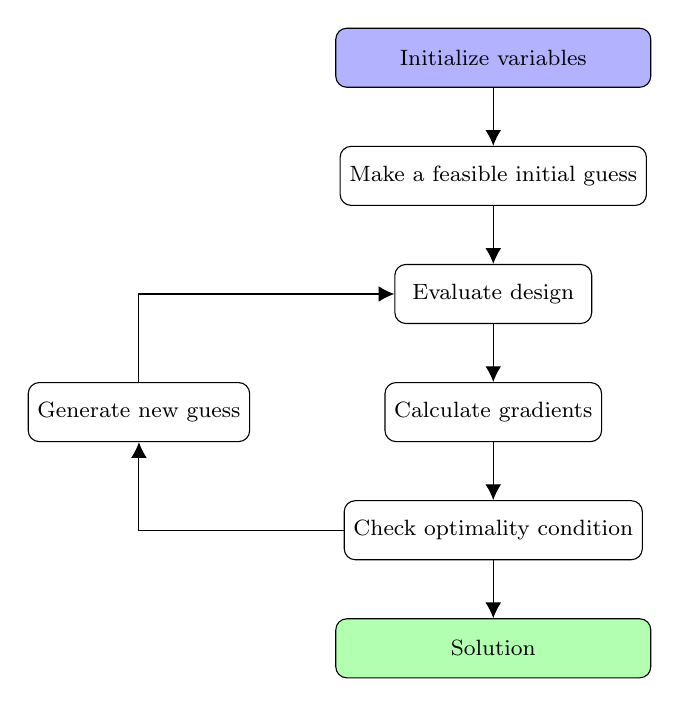
\begin{tikzpicture}[node distance=1.5cm, align=center]
                    \node (start)        [activityStarts]                   {Initialize variables};
                    \node (guess)        [process, below of=start]          {Make a feasible initial guess};
                    \node (evaluate)     [process, below of=guess]          {Evaluate design};
                    \node (gradient)     [process, below of=evaluate]       {Calculate gradients};
                    \node (optimal)      [process, below of=gradient]       {Check optimality condition};
                    \node (solution)     [activityRuns, below of=optimal]   {Solution};
                    \node (genNew)       [process, left of=gradient, xshift=-3cm]        {Generate new guess};

                    \draw[->] (start) -- (guess);
                    \draw[->] (guess) -- (evaluate);
                    \draw[->] (evaluate) -- (gradient);
                    \draw[->] (gradient) -- (optimal);
                    \draw[->] (optimal)  -- (solution);
                    \draw[->] (optimal) -| (genNew);
                    \draw[->]  (genNew) |- (evaluate);
                \end{tikzpicture}}
            \end{center}
            \caption{Gradient-based optimization}
        \end{subfigure}
        \begin{subfigure}[b]{0.5\linewidth}
            \begin{center}
                \resizebox{0.75\textwidth}{!}{
                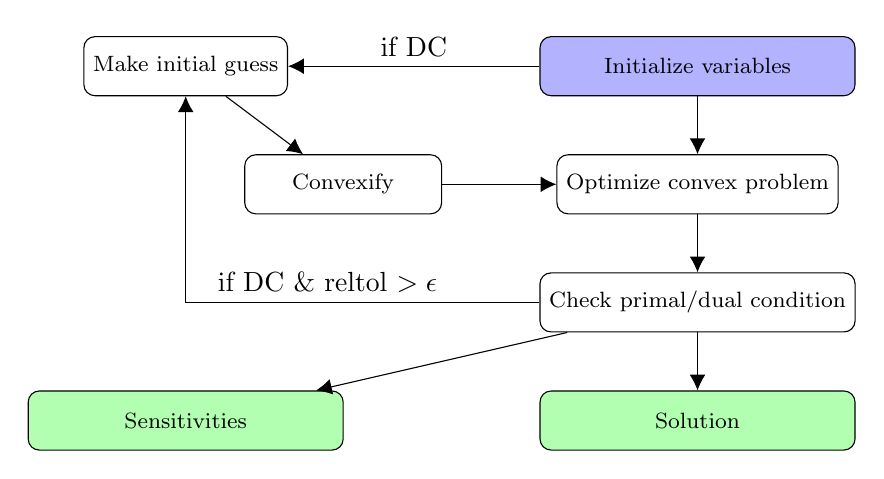
\begin{tikzpicture}[node distance=1.5cm, align=center, scale=0.5]
                    \node (start)        [activityStarts]               {Initialize variables};
                    \node (guess)        [process, left of=start, xshift=-5cm] {Make initial guess};
                    \node (convexify)    [process, below of=guess, xshift=2cm]      {Convexify};
                    \node (optimize)     [process, below of=start]  {Optimize convex problem};
                    \node (condition)    [process, below of=optimize]   {Check primal/dual condition};
                    \node (solution)     [activityRuns, below of=condition]   {Solution};
                    \node (sens)         [activityRuns, left of=solution, xshift=-5cm] {Sensitivities};

                    \draw[->] (start) -- node[yshift=+0.25cm] {if DC} (guess);
                    \draw[->] (start) -- (optimize);
                    \draw[->] (guess) -- (convexify);
                    \draw[->] (convexify) -- (optimize);
                    \draw[->] (optimize) -- (condition);
                    \draw[->] (condition) -| node[yshift=+0.25cm,xshift=1.8cm] {if DC \& reltol $> \epsilon$} (guess);
                    \draw[->] (condition) -- (solution);-
                    \draw[->] (condition) -- (sens);
                \end{tikzpicture}}
            \end{center}
            \caption{Convex, and difference-of-convex (DC) optimization}
        \end{subfigure}
        \caption{The flow diagrams of two methods of optimization.}
        \label{f:optflow}
    \end{figure*}

    A big advantage of convexity is that we can effectively use sensitivity information
    to determine which parts of the
    model yield the greatest returns in terms of fidelity to improved modeling, so engineers can target
    their efforts.

    \item \textit{Models are amenable to mission and multi-point design, and are compatible with modern
    engineering design methodologies.}

    The design tools available in GPkit make it easy to
    implement mission design, and build models that are shared between
    different design problems. Mission design helps engineers gain valuable intuition about
    the tradeoffs in the performance of a design, and multi-point design allows designs to
    be able to satisfy a variety of missions and mission objectives.

\end{enumerate}

This thesis will methodically demonstrate the advantages of \gls{GP} in modeling
and exploring complex engineering trade spaces.




\chapter{Engineering inequalities and intuition, from equalities}
\label{ch2:inequalities}

This section will demonstrate how the form of the \gls{GP} (monomial
equalities and posynomial inequalities) helps engineers gain intuition
about the way that each variable is pressured
by a given objective function. The intuition gained in turn helps formulate
constraints that can properly bound each variable in the model.
GPkit, \gls{CEG}'s \gls{GP} modeling framework,
facilitates process by providing feedback to designers about
the boundedness of a model.

A simple aircraft optimization problem will be derived and will serve as
a demonstration of the intuitive structure of geometric programs, and show
how we can introduce new constraints to bound the feasibility sets of models.

\section{Making feasibility sets and boundedness explicit}

Consider the simple design problem below, where we define a simple bilinear
monomial equality with respect to x and y, and constrain the sum of the variables
to be less than 2:

\begin{equation*}
\begin{aligned}
& {\text{minimize}}
& & x \\
& \text{subject to}
& & x + y \leq 2,
    & & & xy = \frac{1}{2} \label{simple_moneq}
\end{aligned}
\end{equation*}

We can draw the feasibility set of the above problem in both linear and log space,
as shown in Figure~\ref{f:feas_moneq}. One expects that, given only two variables
related through an equality and bounded by inequalities, the feasibility space is
a finite line segment in log-space, and a finite exponential function in linear space.

\begin{figure}
    \centering
    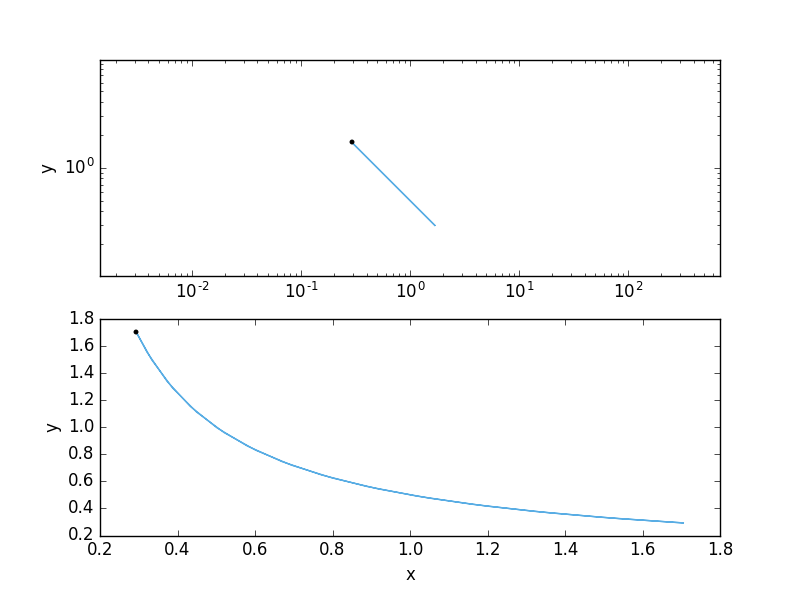
\includegraphics[width=0.8\textwidth]{feas_moneq.png}
    \caption{The x vs y feasibility set of a simple monomial equality.}
    \label{f:feas_moneq}
\end{figure}

However, if we had decided to impose $xy \geq \frac{1}{2}$ instead of $xy = \frac{1}{2}$,
then we would get a new feasibility set as shown in Figure~\ref{f:feas_posygeq}.

\begin{figure}
    \centering
    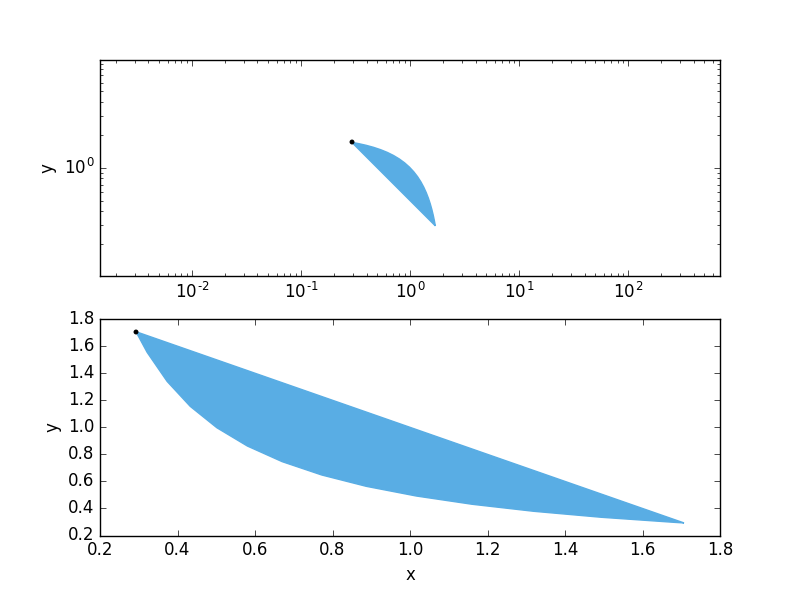
\includegraphics[width=0.8\textwidth]{feas_posygeq.png}
    \caption{The x vs y feasibility set of lower bounding monomial,
    and upper-bonding posynomial.}
    \label{f:feas_posygeq}
\end{figure}

Using the \gls{GP} form, we can always upper-bound posynomials, and lower bound both posynomials
and monomials to get convex feasible sets. Note that the optimal point, which is at
$x = 1 - \frac{1}{\sqrt{2}}$, $y = 1 + \frac{1}{\sqrt{2}}$,
does not change by the relaxation of the monomial equality. This is a key
observation that will allow us to turn most equalities into \gls{GP}-compatible
posynomial inequalities. The posynomial equality relaxation is explained in greater detail
in~\cite{hoburg_thesis}.

However if we convert the monomial equality to  $xy \leq \frac{1}{2}$, we will get an unbounded model,
whose feasibility set is shown in Figure~\ref{feas_posyleq}.

\begin{figure}
    \centering
    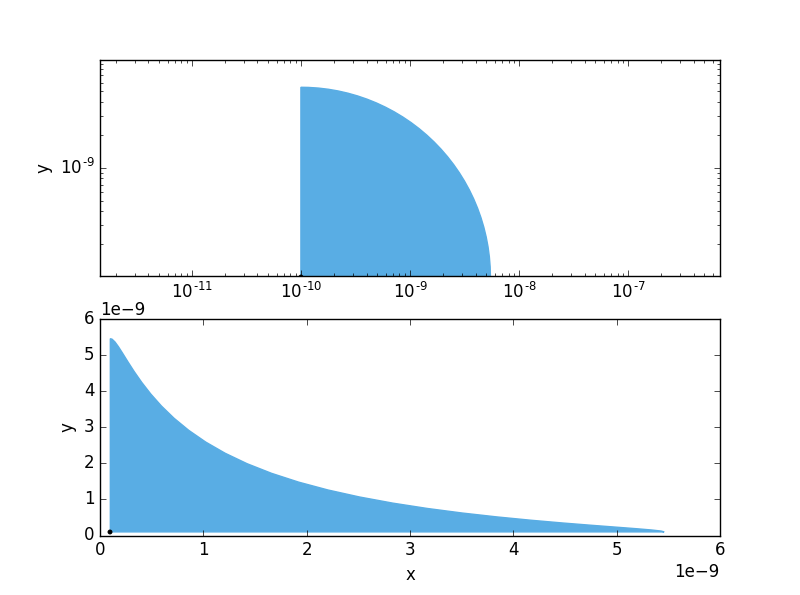
\includegraphics[width=0.8\textwidth]{feas_posyleq.png}
    \caption{The x vs y feasibility set of upper bounding monomial,
    and upper-bonding posynomial.}
    \label{f:feas_posyleq}
\end{figure}

Since $x$ is our objective, and both variables are upper-bounded, they both collapse towards numerical
precision zero,
giving a non-sensical feasibility set shown in Figure~\ref{f:feas_posyleq}. This section will
demonstrate methods to create \gls{GP}-compatible models that are adequately bounded to avoid such
singularities towards zero or infinity, which for the most part do not
exist in real physical models. The models will be created within GPkit~\cite{gpkit}.

\section{Defining the design problem}

\gls{GP}s are amenable to solving a large variety of design problems (see~\cite{gpintro} for an
extensive number of examples). This thesis uses aircraft design to demonstrate
design methodologies that leverage convex optimization since the author's background is in aerospace engineering.
Aircraft epitomize the nature of complex engineering problems. The physical 
relations describing their motion are nonlinear, and all of their subsystems are 
coupled through the primary forces in flight (thrust, weight, lift, drag).
The goal of the aircraft in question will be to perform a basic 'ferry' mission, that
is to carry a given payload
over a distance while minimizing an objective function.

\subsection{Objective functions}
\label{s:objective}

Objective functions are the way that a designer puts pressure on the variables 
in the constraints. To begin with, we will consider
total fuel weight $W_f$ as our objective, which will put
downward pressure on all of the variables that would cause in greater fuel burn, namely
drag and weight. We must necessarily put a lower-bound on all variables expected to
have a positive correlation to the objective function.

In many design problems
formulated as \gls{GP}s, many different objectives will put pressure on design
in the same direction. For example, an aircraft designed for fuel weight will look
different compared to one
that has been designed for total weight or payload-fuel consumption, but all of
these different objective will put a downward pressure on drag and weight.
As such, this model will be able to take in a number of objective functions
and be properly constrained and bounded. According to Raymer, an important
principle of aircraft design is 'that there is no such thing as a free lunch!'
~\cite[pg.26]{raymer}. An improvement in any of the other objective functions
will result in reduced performance with respect to others.

\subsection{Functional description: constraining the problem}

The typical process for designing anything usually involves doing either a
component decomposition or a functional decomposition of the problem. In
this case, we will think about the functional decomposition to create a
basic list of constraints that our aircraft will need to fulfill to be
able to capture the tradeoffs in an aircraft design problem. (In
Section~\ref{s:submodels}, we will examine how thinking about the component decomposition
can help structure larger problems.)

What does an aircraft need to be able to do to deliver payload of a distance?
\begin{itemize}
	\item It will need to sustain steady
    level flight, keeping itself and the payload aloft (Section~\ref{s:wl}).
    \item It will need to overcome drag (Section~\ref{s:td}).
	\item It will need to contain enough fuel to complete its mission
        (Section~\ref{s:fuel}).
	\item It will need to be able to sustain the loads it is
    subjected to (Section~\ref{s:wingstrc}).
\end{itemize}

Note that these are in no way presented in order of importance, which is reflective
of the non-hierarchical nature of \gls{GP}s.
In the basic example, I will choose not to model engines,
and leave this as an exercise
to complete in Section~\ref{s:engine} to improve the model.

\section{GP Modeling from Physics}

Oftentimes, \gls{GP} model creation starts haphazardly, with the designer having a
vague idea about the set of physical a problem, and some basic
set of assumptions about the configuration. In this section, we will
generate variables and constraints with abandon, and think about how to make
sure each variable is adequately bounded later. Each subsection is intended
to introduce the reader to an important aspect of \gls{GP} modeling,
accompanied by examples in implementation.

\subsection{Free and fixed variables: modeling weight and lift}
\label{s:wl}

For this particular design problem, we start by modeling
weight and lift, since the fundamental function of the aircraft is to stay aloft.
The aircraft has weight, which consists of the payload, wing, and fuel weights. 

\begin{equation}
    W \geq W_p + W_w + W_f
\end{equation}

Note that we have already had to make determination about the relations between
the two sides of the equation. Since heavier aircraft burn more fuel, we are justified
to put total weight as greater than the sum of the component weights. Weight relations
are especially amenable to being represented by posynomials, since most objective
functions penalize higher weight.

The aircraft has to sustain steady level flight, which means
that it needs to generate enough lift to carry itself. We use the naive $W \leq L$ 
model below for steady state flight:

\begin{equation}
    W_p + W_w + 0.5 W_f \leq \frac{1}{2} \rho S C_L V^2
\end{equation}

where the lift of the aircraft is equal to weight of the aircraft with half-fuel, 
which is a crude estimate of the average weight of the aircraft throughout the flight.
Again, the \gls{GP} form is seamless here, since lift is related to
induced drag, and so it is pressured downward by the objective function.

We would also like the fully-fueled aircraft to be able to fly at a minimum speed 
of $V_{min}$ without stalling, so we add the following constraint:

\begin{equation}
    W \leq \frac{1}{2} \rho V_{min}^2 S C_{L_{max}}
\end{equation}

Note that, although we could use a monomial equality here, we don't, because this
relation does not need to be tight. It is possible that the aircraft is able to
fly at a velocity slower than $V_{min}$ for a given objective function.

At this point, we have introduced a large set of variables, some of which are input
parameters, and the others free variables. The decision of whether to keep variables free or fixed
can shape the whole model development process in all forms of optimization.
The decision can be influenced by many
factors in a \gls{GP}. In this case, we set the lift coefficient and takeoff speed
to be constants since (1) we would need
more detailed modeling to determine their values. Payload weight is also set
because (2) it would always be unbounded towards zero due to the downward pressure from
the objective. A designer may also fix variables (3) if he/she knows their values with
certainty (eg. gravitational acceleration $g$) or (4) the variable is a normalizing
coefficient (which we will see in Section~\ref{s:datafit}). We will set the values
of some of the variables as defined in Table~\ref{t:vars_WandL}.

\begin{footnotesize}
\begin{table}
    \centering
    \begin{tabular}{ l c l c c}
        \toprule
        Variable & Units & Description & Free & Value \\
        \midrule
        $\rho$ & $~\mathrm{\tfrac{kg}{m^{3}}}$ & density of air & N & 1.23 \\
        $C_L$ & $~\mathrm{-}$ & wing lift coefficient & Y & - \\
        $C_{L,max}$ & $$ & lift coefficient at stall & N &  1.6 \\
        $S$ & $~\mathrm{m^{2}}$ & total wing area & Y & - \\
        $V$ & $~\mathrm{\tfrac{m}{s}}$ & cruising speed & Y & - \\
        $V_{min}$ & $~\mathrm{\tfrac{m}{s}}$ & takeoff speed & N & 25 \\
        $W$ & $~\mathrm{N}$ & total aircraft weight & Y & -\\
        $W_f$ & $~\mathrm{N}$ & fuel weight & Y & -\\
        $W_w$ & $~\mathrm{N}$ & wing weight & Y & - \\
        $W_p$ & $~\mathrm{N}$ & payload weight & N & 6250\\
        \bottomrule
    \end{tabular}
    \caption{Variables introduced in weight vs. lift model. Free variables,
    and constants and their values have been labeled.}
    \label{t:vars_WandL}
\end{table} \end{footnotesize}

Note that the atmospheric variable $\rho$ in Table~\ref{t:vars_TandD}, and other
atmospheric variables in Section~\ref{ch2:inequalities} are set
to be constant. The behavior of these variables with altitude
will be modeled in more detail in Section~\ref{s:mission} when
I model the flight profile of the aircraft.

\subsection{Alternate objective functions: adding performance metrics}
\label{s:altobj}

As multi-objective designers, we may also be interested in knowing about
additional performance metrics that can serve as part of objective functions. A
few that are particularly relevant to aircraft will be introduced here.

The time of flight of the aircraft, which is a useful metric to calculate cost,
is simply the range over velocity:

\begin{equation}
    T_{flight} \geq \frac{\mathrm{Range}}{V}
\end{equation}

The lift-to-drag ratio is also defined: 

\begin{equation}
    L/D = \frac{C_L}{C_D}    
\end{equation}

The new variables we have introduced are detailed in Table~\ref{t:vars_perfMetrics}.

\begin{footnotesize}
\begin{table}
    \centering
    \begin{tabular}{ l c l c c }
        \toprule
        Variable & Units & Description & Free & Value \\
        \midrule
        $C_D$ & $~\mathrm{-}$ & drag coefficient & Y & - \\
        $C_L$ & $~\mathrm{-}$ & wing lift coefficient & Y & - \\
        $L/D$ & $~\mathrm{-}$ & lift-to-drag ratio & Y & - \\
        $Range$ & $~\mathrm{km}$ & aircraft range & N & 3000 \\
        $T_{flight}$ & $~\mathrm{hr}$ & flight time & Y & - \\
        \bottomrule
    \end{tabular}
    \caption{Variables introduced to define new performance metrics.}
    \label{t:vars_perfMetrics}
\end{table} \end{footnotesize}

An important note about variables that are potential alternative objectives: these variables
must always be lower bounded (or inverted and upper bounded) since the general \gls{GP} is a
minimization problem. However, if they are not also upper bounded, these variables
will likely be unbounded for a given model and run off to +$\infty$. This means that
performance-quantifying variables will need to be in a monomial form,
or must be present in a posynomial objective
function as shown in Equation~\ref{e:posyobj} for boundedness.

\begin{equation}
    \mathrm{Objective} \geq \sum\limits^n_{i=1}c_{i}\prod\limits^n_{i=1}  v^{k_{i,j}}
    \label{e:posyobj}
\end{equation}

\subsection{More physics for boundedness: thrust and drag model}
\label{s:td}

If we attempt to run our current model, we would find that it is unbounded in many variables.
The results are shown in Table~\ref{t:WandL_unbounded}.

\begin{footnotesize}
\begin{table}
    \centering
    \begin{tabular}{ l c l }
        \toprule
        Unbounded variable & Units & Direction \\
        \midrule
        $S$ & $~\mathrm{m^{2}}$ & $\infty$ \\
        $T_{flight}$ & $~\mathrm{hr}$ & $\infty$ \\
        $V$ &  $~\mathrm{\tfrac{m}{s}}$  & $\infty$ \\
        $W_f$ & $~\mathrm{N}$ & $0$ \\
        $W_w$ & $~\mathrm{N}$  & $0$ \\
        \bottomrule
    \end{tabular}
    \caption{Unbounded variables in the weight and lift model. More modeling, or direct
    substitutions are required.}
    \label{t:WandL_unbounded}
\end{table} \end{footnotesize}

This is not surprising at all, since none of the defined variables lower bound $W_f$,
the objective function, in the constraints we have defined.
Without the pressure from the objective, any variables that
are not both upper- and lower- bounded will tend to blow up. This is indicative usually
that more modeling or direct substitutions are required to sufficiently bound the variables.

In this case, we lack a propulsion model which would properly bound fuel weight, velocity,
and time of flight. For initial modeling purposes, I assume a naive constant brake
specific fuel consumption (\BSFC) for the 'engine' of the aircraft, which is assumed
to provide as much thrust as needed. Since $T \geq D$:

\begin{equation}
    W_f \geq \BSFC \times T_{flight} \times D
    \label{e:W_f}
\end{equation}

the fuel weight required is the product of the \BSFC, time of flight, and the
total drag on the aircraft.
The drag of the aircraft is the product of dynamic pressure ($\frac{1}{2} \rho V^2$),
the planform area $S$, and the coefficient of drag of the aircraft:

\begin{equation}
    D \geq \frac{1}{2} \rho V^2 S C_D
    \label{e:d}
\end{equation}

There are yet more relaxed monomial equalities in Equations~\ref{e:W_f} and \ref{e:d}.
If the pressure on the \gls{LHS} or \gls{RHS} of a monomial equality are clear as in these cases,
it is a good practice to relax the equality to leave as many degrees of freedom
in the design space as possible. The intuition is that, we can almost always spend more fuel or have more drag,
but the constraints will always be tight since all objectives will suffer as a consequence.

The drag coefficient of the aircraft is assumed to be the sum of the fuselage drag,
the wing profile drag, and the wing induced drag coefficients \cite{gp_ac_design}:

\begin{equation}
    C_D \geq C_{D_{fuse}} + C_{D_{wpar}} + C_{D_{ind}}
\label{e:cd}
\end{equation}

The individual components of the drag are represented as monomial equalities, again borrowing
from \cite{gp_ac_design} for constraints~\ref{e:cdfuse} through~\ref{e:cdinduced}.
The fuselage drag is a function of its drag area $CDA_0$ and the planform area of the wing:

\begin{equation}
    C_{D_{fuse}} = \frac{CDA_0}{S}
\label{e:cdfuse}
\end{equation}

where the $CDA_0$ is linearly proportional to the volume of fuel in the fuselage:

\begin{equation}
    V_{f_{fuse}} = CDA_0 \times 10 ~\mathrm{[meters]}
\label{e:vffuse}
\end{equation}

Note that we correct the dimensionality of the volume here, since GPkit automatically checks units.

The wing profile drag is the product of the form factor, the friction drag coefficient,
and the wetted area ratio of the wing \cite{gp_ac_design},

\begin{equation}
    C_{D_{wpar}} = k C_f S_{wetratio}
\label{e:cdwpar}
\end{equation}

The Reynolds number of the aircraft wing is approximated

\begin{equation}
    Re \leq \frac{\rho}{\mu} V \sqrt{\frac{S}{\AR}}
\label{e:re}
\end{equation}

and used to find the friction drag coefficient of wing. We approximate the $C_f$ by assuming a
turbulent Blasius flow over a flat plate as below:

\begin{equation}
    C_f \geq \frac{0.074} {Re^{0.2}}
\end{equation}

The induced drag of the wing is calculated with a span efficiency factor e, and is a
function of the $C_L$ and aspect ratio $AR$ of the wing.

\begin{equation}
    C_{D_{induced}} = \frac{C_L^2}{\pi \AR e}
\label{e:cdinduced}
\end{equation}

The new variables are detailed in Table~\ref{t:vars_TandD}.

\begin{footnotesize}
\begin{table}
    \centering
    \begin{tabular}{ l c l c c }
        \toprule
        Variable & Units & Description & Free & Value \\
        \midrule
        $A$ & $-$ & aspect ratio & Y & - \\
        $\BSFC$ & $\mathrm{\frac{g}{kW*hr}}$ & brake specific fuel consumption & N & 400 \\
        $(CDA0)$ & $~\mathrm{m^{2}}$ & fuselage drag area & Y & - \\
        $C_f$ & $-$ & skin friction coefficient & Y & - \\
        $D$ & $~\mathrm{N}$ & total drag force & Y & - \\
        $e$ & $-$ & Oswald efficiency factor & N & 0.92 \\
        $k$ & $-$ & form factor & N & 1.17 \\
        $\mu$ & $~\mathrm{\tfrac{kg}{m\cdot s}}$ & viscosity of air & N &
            $\mathrm{1.78 \times 10^{-5}}$ \\
        $Re$ & $-$ & Reynolds number & Y & - \\
        $\left(\frac{S}{S_{wet}}\right)$ & $-$ & wetted area ratio & N & 2.075 \\
        $V_{f_{fuse}}$ & $~\mathrm{m^{3}}$ & fuel volume in the fuselage & Y & - \\
        \bottomrule
    \end{tabular}
    \caption{Variables introduced in thrust and drag model.}
    \label{t:vars_TandD}
\end{table} \end{footnotesize}

%\begin{python}
%        # Thrust and drag model
%        C_D_fuse = CDA0 / S
%        C_D_wpar = k * C_f * S_wetratio
%        C_D_ind  = C_L ** 2 / (np.pi * A * e)
%        constraints += [W_f >= BSFC * T_flight * D,
%                    D >= 0.5 * rho * S * C_D * V ** 2,
%                    C_D >= C_D_fuse + C_D_wpar + C_D_ind,
%                    V_f_fuse == 10*units('m')*CDA0,
%                    Re <= (rho / mu) * V * (S / A) ** 0.5,
%                    C_f >= 0.074 / Re ** 0.2]
%\end{python}

As shown in Table~\ref{t:WLTD_unbounded} attempting to run the model as is
results in both the fuselage fuel
volume $V_{f_{fuse}}$ and the wing weight $W_w$ still being lower-unbounded.
These variables will need to be properly bounded to complete the SimPleAC model.

\begin{footnotesize}
    \begin{center}
        \begin{table}
            \begin{tabular}{ l c l }
                \toprule
                Unbounded variable & Units & Direction \\
                \midrule
                $V_{f_{fuse}}$ &  $~\mathrm{m^3}$  & $0$ \\
                $W_w$ & $~\mathrm{N}$  & $0$ \\
                \bottomrule
            \end{tabular}
            \caption{Unbounded variables within the GP formulation}
            \label{t:WLTD_unbounded}
        \end{table}
    \end{center}
\end{footnotesize}

\section{Limits of GP and Convexity, and SP modeling} \label{s:GPLimits}

Even with the demonstrated strengths of \gls{GP}'s in solving certain classes of 
problems, it is important to recognize that the mathematical framework has limits. 
Certain constraints can only be expressed as signomial constraints, which are 
difference-of-posynomial constraints. Even the addition of a single
signomial constraint turns the problem from a \gls{GP} to a \gls{SP}, which means
that the problems loses convexity and all of the mathematical guarantees associated with it. 
It takes engineering intuition to recognize where and when improved modeling is worth
the loss of the mathematical guarantees.

\subsection{Signomial constraints: adding fuel volume model}
\label{s:fuel}

In an attempt to lower bound $V_{f_{fuse}}$, we will
be adding a fuel volume model to SimPleAC, where fuel can be stored in the wing or
in the fuselage. The fuel volume will be modeled first instead of the wing
weight because the wing weight will be a function of the fuel stored in the fuselage.
The reason why this model is \gls{GP}-incompatible is because of the
following constraint which follows logically:

\begin{equation}
	V_{f_{avail}} \leq V_{f_{wing}} + V_{f_{fuse}}
	\label{vfavail}
\end{equation}

The fuel volume available must be less than the sum of the fuel volume available in the
wing and the fuselage. It turns out that volumes that 'contain' free variables
can create signomial constraints. (One way around this is potentially creating fuel
fraction variables to denote how much fuel is stored in each volume, but
other potential parametrizations will not be explored here.)

As such, we can continue to develop the model, since it is important for us to
capture the fuel distribution between the wing and the fuselage. Fuel weight is going
to influence the lift required of the aircraft, so the weight of the fuel is determined
using a density parameter $\rho_{f}$. 

\begin{equation}
    V_f = \frac{W_f } {\rho_f g}
    \label{e:vf}
\end{equation}

We need a model of how much fuel volume there is in a wing. Intuitively,
we would expect the volume within a wing
to be related linearly to its thickness ratio ($\tau$) and span ($b$),
and to the square of its chord ($c$). 

\begin{equation}
	V_{f_{wing}} \propto \tau b c^2
	\label{e:vfwingpre}
\end{equation} 

In aerospace engineering, we like dimensionless quantities and planform areas, 
so we would like to express relation~\ref{e:vfwingpre} with respect to the planform area $S$
aspect ratio \AR and thickness ratio $\tau$ only, without having to define $b$ and $c$ as new
free variables.
Using the additional relations $\AR = \frac{b^2}{S}$ and $S \propto b c$, we can
express $V_{f_{wing}}$.

\begin{equation}
	V_{f_{wing}} \propto \tau (\frac{\AR}{S})^{0.5} (\frac{S}{b})^2 \propto
		(\frac{\AR}{S})^{0.5} \frac{S^2}{S \AR} \propto \frac{\sqrt{S}\tau}{\sqrt{\AR}}
\end{equation}

\begin{equation}
\label{e:vfwing}
V_{f_{wing}}^2 \leq 9\times10^{-4} \frac{S \tau^2}{\AR}
\end{equation}

Such variable transformations can be useful to have a minimal parametrization of designs.
One can solve the minimal problem, and
post-process the results of the optimization problem to get complete geometry
as necessary. The new variables introduced to bound fuel volume are in Table~\ref{t:vars_fuelmodel}.
(In the final form of the Equation~\ref{e:vfwing} the constant $9\times10^{-4}$ was picked as the coefficient in
front of the relation by tuning it after the model was developed,
but any other coefficient would work.)

\begin{footnotesize}
\begin{table}
    \centering
    \begin{tabular}{ l c l c c }
        \toprule
        Variable & Units & Description & Free & Value \\
        \midrule
        $\rho_f$ & $~\mathrm{\tfrac{kg}{m^{3}}}$ & density of fuel & N & 817 \\
        $g$ & $~\mathrm{\tfrac{m}{s^{2}}}$ & gravitational acceleration & N & 9.81 \\
        $\tau$ & $$ & airfoil thickness to chord ratio & N & 0.12 \\
        $V_f$ & $~\mathrm{m^{3}}$ & fuel volume & Y & - \\
        $V_{f_{avail}}$ & $~\mathrm{m^{3}}$ & fuel volume available & Y & - \\
        $V_{f_{wing}}$ & $~\mathrm{m^{3}}$ & fuel volume in the wing & Y & - \\
        \bottomrule
    \end{tabular}
    \caption{Variables introduced in the fuel model.}
    \label{t:vars_fuelmodel}
\end{table} \end{footnotesize}

\subsection{Arguments for the signomial equality}
\label{s:sigeq}

This segue will explain and motivate the use of signomial equalities,
as described in~\cite{sigeqpaper}, in \gls{SP} modeling.
Signomial equalities must be used as a last resort. The signomial equality is the only place
where the feasibility set of individual \gls{GP}'s within a \gls{SP} solve are not guaranteed
to be subsets of the feasibility set of the \gls{SP}. This is because the signomial solution
algorithm in GPkit flattens the original signomial equality constraint,
a concave curve in log-space in n-dimensions,
onto a line in log-space in n-dimensions(Method C in~\cite{sigeqpaper}) that intersects the
original constraint at the optimal point of the last \gls{GP} solve. This is undesirable although
the final solution of the \gls{SP} with equalities
is guaranteed to be in the feasibility region of the \gls{SP}. Furthermore, \gls{SP}s
with signomial equalities have been demonstrated to require more \gls{GP} solves
than \gls{SP}s without signomial equalities. However, there are a few arguments
to be made in defense of signomial equalities.

One good use case of the signomial equalities is in constraints in which the direction
of pressure on free variables is not clear. This ensures the tightness of constraints
that may otherwise have unbounded variables. A good example is in atmospheric models.
Although the pressure on air density $\rho$ is almost certainly downward since it results in
lower drag, the pressure on viscosity $\mu$ is not clear because of the complex relationship
between Reynolds number and drag.

The second reason is that we are not interested in the 'feasibility set' of the atmosphere,
since this has no intuition behind it: at every altitude, the atmospheric quantities
can only be be represented by single quantities. Additionally, the computational penalty of
implementing signomial equalities in atmospheric models is low, since the monomial approximation
to the atmospheric data is not far from the monomial approximations made to the signomial equality.
In fact, when we add an atmospheric model to SimPleAC in
Section~\ref{s:mission}, we will be implementing signomial equalities to represent both air density
$\rho$ and viscosity $\mu$.

\subsection{Completing the model: wing structural model}
\label{s:wingstrc}

Only one unbounded variable remains, which is wing weight $W_w$. We can think
of wing weight having two components, the skin weight that
only grows as a function of wing area, the structural weight which is a function of
both the geometry and loading. The surface weight expression is straightforward.

\begin{equation} W_{w_{surf}} \geq W_{w_{coeff2}} S \label{e:wwsurf} \end{equation}

We would like wing structural weight to account for the loading distribution and the geometry
of the wing. The wing will have to sustain a maximum bending load (I will neglect shear, since
the two are coupled) due to maximum takeoff weight,
multiplied by an ultimate structural factor $N_{ult}$ for maneuvering.
I have borrowed the wing weight model from \cite{gp_ac_design}, and adapted it through a
structural weight coefficient $W_{w_{coeff1}}$. Note that this equation captures the
major trends in wing structural sizing. We can see this through looking at the partial
derivatives of the wing weight with respect to the different free variables.
The weight grows with the cube of the span ($AR^{1.5} = \frac{b^3}{S_{constant}^{1.5}}$, derived
from the integration of a quadratically increasing bending moment),
linearly with the maximum structural factor $N_{ult}$, and inversely with the
surface area \footnotemark. Using similar partial-derivative based analyses, it
is often easy to make first-order models for components.

\footnotetext{This can be difficult to see, but since $S \propto b_{constant} c$ and loading is constant, as area
grows, the thickness of the wing grows as well at a constant $\tau$. So the weight increases linearly with S,
and stiffness increases with the cube of S.
Integrated over the whole wing this yields a $S^{-1}$ relation.}

\begin{equation} W_{w_{strc}} \geq \frac{W_{w_{coeff1}}}{\tau}
N_{ult} AR ^ {1.5} \sqrt{(W_0+\rho_fgV_{f_{fuse}}) WS} \label{e:wwstrc}
\end{equation}

Equation~\ref{e:wwstrc} takes into account the root
bending moment relief due to presence of fuel and weight in the wings by performing a
geometric average of the total weight, and the weight excluding wing fuel and wing weight.

The total wing weight is now lower-bounded by its component weights, and we have introduced
the final set of variables in Table~\ref{t:vars_wingstrcmodel}.

\begin{equation} W_w \geq W_{w_{surf}} + W_{w_{strc}} \label{e:ww} \end{equation}

\begin{footnotesize}
\begin{table}
    \centering
    \begin{tabular}{ l c l c c }
        \toprule
        Variable & Units & Description & Free & Value \\
        \midrule
        $N_{ult}$ & $-$ & ultimate load factor & N & 3.3 \\
        $W_{w_{coeff1}}$ & $~\mathrm{\tfrac{1}{m}}$ & wing weight coefficient 1 & N &
                $\mathrm{2\times 10^{-5}}$ \\
        $W_{w_{coeff2}}$ & $~\mathrm{Pa}$ & wing weight coefficient 2 & N & 60 \\
        $W_{w_{strc}}$ & $~\mathrm{N}$ & wing structural weight & Y & - \\
        $W_{w_{surf}}$ & $~\mathrm{N}$ & wing skin weight & Y & - \\
    \bottomrule
    \end{tabular}
    \caption{Variables introduced in the wing structural model.}
    \label{t:vars_wingstrcmodel}
\end{table} \end{footnotesize}

\section{Results of SimPleAC}

The benefits of convex optimization and \gls{GP} in both solution
quality (in terms of mathematical guarantees) and the low-cost
computation of sensitivities has been detailed in (\cite{gp_ac_design},\cite{sp_ac_design}),
so these benefits will not be featured here. However, the values of the free variables,
and the sensitivities of the fixed parameters are presented for the reader.

\begin{center}
\captionof{table}{Values of the free variables in the SimPleAC model.}
% \documentclass[12pt]{article}
% \usepackage{booktabs}
% \usepackage{longtable}
% \usepackage{amsmath}
% \begin{document}

{\footnotesize
\begin{longtable}{llc}
\toprule
Free Variables & Value & Units \\ \midrule
$(CDA0)$ & 0.004751  & $~\mathrm{m^{2}}$ \\
$A$ & 23.41  & $$ \\
$C_D$ & 0.01928  & $$ \\
$C_L$ & 0.7867  & $$ \\
$C_f$ & 0.004054  & $$ \\
$C_{D_{fuse}}$ & 0.0002902  & $$ \\
$C_{D_{ind}}$ & 0.009149  & $$ \\
$C_{D_{wpar}}$ & 0.009843  & $$ \\
$D$ & 237.2  & $~\mathrm{N}$ \\
$L/D$ & 40.8  & $$ \\
$Re$ & 2.026e+06  & $$ \\
$S$ & 16.37  & $~\mathrm{m^{2}}$ \\
$T_{flight}$ & 23.84  & $~\mathrm{hr}$ \\
$V$ & 34.96  & $~\mathrm{\tfrac{m}{s}}$ \\
$V_f$ & 0.09678  & $~\mathrm{m^{3}}$ \\
$V_{f_{avail}}$ & 0.09678  & $~\mathrm{m^{3}}$ \\
$V_{f_{fuse}}$ & 0.04751  & $~\mathrm{m^{3}}$ \\
$V_{f_{wing}}$ & 0.04928  & $~\mathrm{m^{3}}$ \\
$W$ & 1.007e+04  & $~\mathrm{N}$ \\
$W_f$ & 775.7  & $~\mathrm{N}$ \\
$W_w$ & 3041  & $~\mathrm{N}$ \\
$W_{w_{strc}}$ & 2059  & $~\mathrm{N}$ \\
$W_{w_{surf}}$ & 982.1  & $~\mathrm{N}$ \\
\bottomrule
\end{longtable}}

% \end{document}

% \end{document}

    \label{t:SimPleAC_results}
\end{center}

\begin{center}
\captionof{table}{Sensitivities of parameters in the SimPleAC model.}
% \documentclass[12pt]{article}
% \usepackage{booktabs}
% \usepackage{longtable}
% \usepackage{amsmath}
% \begin{document}

{\footnotesize
\begin{longtable}{llc}
\toprule
Sensitivities & Value & Units \\ \midrule
$\BSFC$ & +1.1  & $~\mathrm{\tfrac{g}{\left(hr\cdot kW\right)}}$ \\
$Range$ & +1.1  & $~\mathrm{km}$ \\
$W_p$ & +1.1  & $~\mathrm{N}$ \\
$g$ & +1.1  & $~\mathrm{\tfrac{m}{s^{2}}}$ \\
$\left(\frac{S}{S_{wet}}\right)$ & +0.57  & $$ \\
$k$ & +0.57  & $$ \\
$e$ & -0.53  & $$ \\
$V_{min}$ & -0.49  & $~\mathrm{\tfrac{m}{s}}$ \\
$\tau$ & -0.34  & $$ \\
$N_{ult}$ & +0.31  & $$ \\
$W_{w_{coeff1}}$ & +0.31  & $~\mathrm{\tfrac{1}{m}}$ \\
$\rho$ & -0.3  & $~\mathrm{\tfrac{kg}{m^{3}}}$ \\
$C_{L,max}$ & -0.24  & $$ \\
$W_{w_{coeff2}}$ & +0.15  & $~\mathrm{Pa}$ \\
$\mu$ & +0.11  & $~\mathrm{\tfrac{kg}{\left(m\cdot s\right)}}$ \\
$\rho_f$ & -0.044  & $~\mathrm{\tfrac{kg}{m^{3}}}$ \\
\bottomrule
\end{longtable}}

% \end{document}

% \end{document}

    \label{t:SimPleAC_sens}
\end{center}




\chapter{Extensibility of GP}
\label{ch3:extensibility}

Recalling from Figure~\ref{f:optflow}, traditional gradient-based design optimization tools implement
convergence loops that assume structure within a given design problem.
The 'bag of constraints' form of the GP means that constraints can be
added to the problem without
having to restructure the optimization formulation. This property,
coupled with the object-oriented modeling framework of GPkit, allows
\gls{GP} compatible models to be continuously extensible.
This section will demonstrate common methods used to extend the capability
and improve the fidelity of \gls{GP}- and \gls{SP} compatible models.

\section{Improving fidelity: Adding a simple engine model to the SimPleAC}
\label{s:engine}

The SimPleAC currently has an engine that weighs nothing and magically supplies
unlimited power. This is obviously unphysical, and requires refinement.

\subsection{Creating an engine submodel}

Before even thinking about modeling, we would like to leverage the object-oriented
GPkit models to put the variables describing the engine into a submodel (currently only
BSFC). We do this by creating a new class called \textbf{Engine} and creating a \textit{setup}
method that returns the constraints within it.

\begin{python}
    class Engine(Model):
        def setup(self):
            # Dimensional constants
            BSFC = Variable("BSFC", 400, "g/(kw*hr)", "brake specific fuel consumption")
            constraints = []
            return constraints
\end{python}

We allow the SimPleAC model to contain the variables and constraints of the engine
as follows:

\begin{python}
    class SimPleAC(Model):
        def setup(self):
            self.engine = Engine()
            self.components = [self.engine]
            ...
            return constraints, self.components
\end{python}

This restructuring of the model yields the exact same overall \gls{GP} formulation
as the unstructured problem, but gives us the flexibility to develop submodels
collaboratively and in a disciplined manner.

If we think of an engine as an input-output system, we can determine how it
would interact with the SimPleAC system, and create appropriately bounded
sets of variables.
At the most basic level, the engine provides shaft power, consumes fuel,
and has weight. The model is missing both the shaft power and weight description
of the engine. If we abstract away the propeller (the relation between shaft
power and thrust power) through a propeller efficiency,
we can perhaps relate maximum power to weight.

\subsection{Data-based modeling: engine power vs. weight}
\label{s:datafit}

We can imagine that, for a specific kind of engine, there is a relation between the
maximum shaft power available and the mass of the engine, somewhat related to the
cube-square law, which describes the relation between the surface area and volume
of objects. And let's assume that our knowledge of the internal workings of engines
is limited, but we have some knowledge of the technology available in the market
and have data to support it. Using GPfit~\cite{gpfitpaper}, we will try to fit the data to find
\gls{GP} compatible relations between engine weight and maximum power. This section
will try to highlight the best practices when making data-based models.

To be able to fit the engine power vs. weight data, we take several important steps.
\begin{itemize}
    \item \textbf{Comb the data.} Since we are essentially projecting
    data with potentially high standard deviation onto a single line,
    it is important to fit the ranges of data we care about.
    \item \textbf{Normalize the data.} Normalizing the data
    by some known quantity is preferable, fits should not be dependent on the
    units that are used while performing it. This also helps the fit integrate
    seamlessly into GPkit, since dimensional fits would require units manipulation
    to avoid errors. The data can be normalized by any
    reference quantities (in this case using the maximum power and weight values
    from the data set).
    \item \textbf{Choose the type of fit.} In~\cite{gpfitpaper}, \textit{softmax-affine}
    (SMA) and \textit{implicit softmax-affine} (ISMA)
    functions are proposed and implemented as convex approximations
    to data. Depending on the behavior of the data, one or the other
    may be appropriate. For engineering relations that are expected to be smooth, SMA
    functions are often good approximations. However, if kinks are expected in the
    functions, ISMA functions can locally adjust the softness of the fit to
    reduce the error of the fit.
    \item \textbf{Choose the number of posynomial terms in the fit.} The number of
    terms will likely depend on the root-mean square (RMS) error of the fit, and
    the kind of pressure on the variable. RMS error can be reduced by including
    more posynomial terms, but only if the variable of interest has downward
    pressure on it from the objective function (since it is on the greater side
    of the inequality).
\end{itemize}

After having performed these intermediate steps on the engine data,
the relation we obtain for the one-term (monomial) approximation is as follows:

\begin{equation}
    \left(\frac{W_{eng}}{W_{eng,max}}\right)^{0.100} = 0.988 \left(\frac{P_{shaft}}{P_{shaft,max}}\right)^{0.117}
\end{equation}

Note that the root mean square error of this fit is 0.414, which primarily has to do with
the level of variation in the data. Since engine weight will have downward pressure
on it from the objective, we can easily use a two-term posynomial approximation to
improve its error.

\begin{equation}
    \left(\frac{W_{eng}}{W_{eng,max}}\right)^{0.801} \geq 0.0330 \left(\frac{P_{shaft}}{P_{shaft,max}}\right)^{0.167}
    +1.59 \left(\frac{P_{shaft}}{P_{shaft,max}}\right)^{1.36}
\end{equation}

This relation has an r.m.s. error of 0.346, which is a significant improvement.
Both fits are shown with the data in Figure~\ref{f:enginefit}.

\begin{figure}
    \centering
    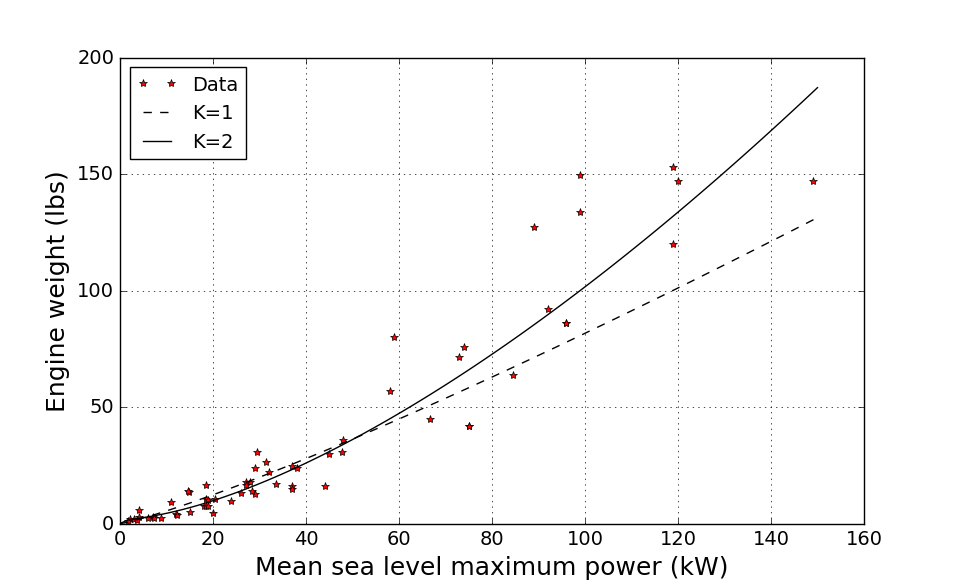
\includegraphics[width=0.6\textwidth]{enginePvsW.png}
    \caption{Engine MSL power versus weight fits for $K=1,2$ posynomial terms with underlying data.}
    \label{f:enginefit}
\end{figure}

With a SMA approximation, more terms do not improve the r.m.s.
error of the fit on the given data, due to the large standard deviation of the data used.
As such, we will proceed with the 2-term posynomial fit.

\subsubsection{Other constraints in engine model}

The cruise shaft power is constrained to be 20\% of the maximum shaft power of the engine,
to account for engine surge power demands and add engineering realism. This rather arbitrary constraint is removed
later when the full mission model is integrated.

\begin{equation}
    P_{shaft} \leq \frac{1}{5} P_{shaft,max}
\end{equation}

\subsection{Converting all subsystems into submodels}
\label{s:submodels}

Within this framework, we can modularize the SimPleAC into wing and fuselage modules as well,
with very little additional work. This creates the variable and constraint
hierarchy as presented in Figure~\ref{forest:submodels}, which define all of the constraints
required for SimPleAC to fly one flight segment.

\begin{figure}[!h]
    \centering\small\sffamily
    \begin{forest}
        sn edges
        [\textbf{Aircraft}
        [\textbf{Wing}]
        [\textbf{Fuselage}]
        [\textbf{Engine}]
        ]
    \end{forest}
    \caption{Variable and constraint hierarchy of the single mission segment SimPleAC model}
    \label{forest:submodels}
\end{figure}

Tree or graph structures such as in Figure~\ref{forest:submodels} are informative, since
it provides an intuitive representation of the way constraints and variables
are passed between GPkit models. Due to the serial nature of object creation in software engineering,
variables and constraints from one model can only be called by models that are higher in the tree diagram.


The way the \gls{SP} is solved at the end has no
hierarchy, but as we will see in Section~\ref{s:mission} a hierarchical representation
will facilitate the vectorization of constraints required for mission design.

%TODO: develop on the idea of variable and constraint hierarchy

\section{Mission design and performance modeling form}
\label{s:mission}

The SimPleAC defined so far works well to demonstrate the
capabilities of \gls{SP} in helping explore tradeoffs in engineering design.
However, often in the design process, we will want to test the performance of a
design in different conditions, and/or during different phases of a mission.
This requires the vectorization of
constraints that relate to the performance of the design. What we'd like to do
is to have a single aircraft optimize both its static sizing variables (having
to do with the airframe), and its flight performance simultaneously. This requires a major
augmentation of the model tree defined in Figure~\ref{forest:submodels}, into a
uni-directional graph as shown in Figure~\ref{f:missiongraph}.

\begin{figure}[!h]
    \centering\small\sffamily
    \begin{forest}
        sn edges,
        l sep+=1em,
        for children={
        l sep+=1em,
        }
        [\textit{\textbf{Mission}},name=mission
        [\textit{\textbf{\shortstack{Aircraft\\Perf.}}},name=aircraftP2
        [\textit{\shortstack{Wing\\Perf.}},name=wingP2]
        [\textit{\shortstack{Engine\\Perf.}},name=engineP2
        [\textit{Atmosphere},name=atmos2]]]
        [,name=phantom
        [\textbf{Aircraft},name=aircraft
        [\textbf{Wing},name=wing]
        [\textbf{Fuselage},name=fuse]
        [\textbf{Engine},name=engine]
        ]]
        [\textit{\textbf{\shortstack{Aircraft\\Perf.}}},name=aircraftP1
        [\textit{\shortstack{Wing\\Perf.}},name=wingP1]
        [\textit{\shortstack{Engine\\Perf.}},name=engineP1
        [\textit{Atmosphere},name=atmos1]]
        ]
        ]
        \draw[->] (atmos1) -- (wingP1);
        \draw[->] (atmos1) -- (aircraftP1);
        \draw[->] (atmos2) -- (wingP2);
        \draw[->] (atmos2) -- (aircraftP2);
        \draw[->] (aircraft) -- (aircraftP1);
        \draw[->] (aircraft) -- (aircraftP2);
        \draw[->] (wing) -- (wingP1);
        \draw[->] (engine) -- (engineP1);
        \draw[->] (wing) -- (wingP2);
        \draw[->] (engine) -- (engineP2);
        \node[draw,rectangle,fit={(aircraftP2) (atmos2) (engineP2) (wingP2)}] {};
        \node[draw,rectangle,fit={(aircraftP1) (atmos1) (engineP1) (wingP1)}] {};
    \end{forest}
    \caption{Variable and constraint hierarchy of the presented aircraft model, for two flight
    segments. Models that include sizing variables are
    bolded while models that include performance variables are italicized.
    There are models that contain both kinds of variables.}
    \label{f:missiongraph}
\end{figure}

Figure~\ref{f:missiongraph} represents a model with two flight segments, where the
models enclosed in rectangles contain the set of constraints that are vectorized
by the number of flight segments, $N_{segments} = 2$. Each
one of the performance models contain variables that change between flight segments.
Note that the fuselage is the only subcomponent not to have a performance model.
This is because the only performance variable of the fuselage is its drag
coefficient, which is assumed to not change between flight segments, making it static. I
have also added a \textbf{\textit{Mission}} model, which links flight segments together,
and an \textit{Atmosphere} model, which describes the conditions in which the aircraft
operates.

The static aircraft model, and the atmospheric state are passed as an argument to multiple
performance models within this framework. To transform our previously static model to
the performance-static model hierarchy we have identified,
we have to determine which variables
belong in which node of the tree. Table~\ref{t:missionvars} details the full
decomposition of the model into its submodels in the format defined
by Figure~\ref{f:missiongraph}. This is as simple as identifying which variables
we do not expect to change during flight segments, and which ones we do.

\begin{center}
    \captionof{table}{Variables of SimPleAC in performance modeling, detailed in the
    variable and constraint hierarchy.}
    {\footnotesize
\begin{longtable}{lcl}
\toprule
Free Variables & Units & Description \\ \midrule
\multicolumn{3}{l}{\textbf{Mission}} \\
$W_{f_{m}}$ & $~\mathrm{N}$ & Total mission fuel \\
$t_m$ & $~\mathrm{hr}$ & Total mission time \\
$R_s$ & $~\mathrm{km}$ & Range flown in segment \\
$W_{avg}$ & $~\mathrm{N}$ & Segment average weight \\
$W_{end}$ & $~\mathrm{N}$ & Weight at the end of flight segment \\
$W_{f_s}$ & $~\mathrm{N}$ & Segment fuel burn \\
$W_{start}$ & $~\mathrm{N}$ & Weight at the beginning of flight segment \\
$\frac{\Delta h}{dt}$ & $~\mathrm{\tfrac{m}{hr}}$ & Climb rate \\
$h$ & $~\mathrm{m}$ & Flight altitude \\
$t_s$ & $~\mathrm{hr}$ & Time spent in flight segment \\
\hline
\multicolumn{3}{l}{\textbf{Mission/Atmosphere}} \\
$\mu$ & $~\mathrm{\tfrac{kg}{\left(m\cdot s\right)}}$ & dynamic viscosity \\
$\rho$ & $~\mathrm{\tfrac{kg}{m^{3}}}$ & density of air \\
$h$ & $~\mathrm{m}$ & altitude \\
\hline
\multicolumn{3}{l}{\textbf{Mission/SimPleAC}} \\
$V_f$ & $~\mathrm{m^{3}}$ & maximum fuel volume \\
$V_{f_{avail}}$ & $~\mathrm{m^{3}}$ & fuel volume available \\
$W$ & $~\mathrm{N}$ & maximum takeoff weight \\
$W_f$ & $~\mathrm{N}$ & maximum fuel weight \\
\hline
\multicolumn{3}{l}{\textbf{Mission/SimPleAC/Engine}} \\
$P_{shaft_{max}}$ & $~\mathrm{kW}$ & MSL maximum shaft power \\
$W_e$ & $~\mathrm{N}$ & engine weight \\
\hline
\multicolumn{3}{l}{\textbf{Mission/SimPleAC/Fuselage}} \\
$(CDA0)$ & $~\mathrm{m^{2}}$ & fuselage drag area \\
$C_{D_{fuse}}$ & $$ & fuselage drag coefficient \\
$V_{f_{fuse}}$ & $~\mathrm{m^{3}}$ & fuel volume in the fuselage \\
\hline
\multicolumn{3}{l}{\textbf{Mission/SimPleAC/Wing}} \\
$A$ & $$ & aspect ratio \\
$S$ & $~\mathrm{m^{2}}$ & total wing area \\
$V_{f_{wing}}$ & $~\mathrm{m^{3}}$ & fuel volume in the wing \\
$W_w$ & $~\mathrm{N}$ & wing weight \\
$W_{w_{strc}}$ & $~\mathrm{N}$ & wing structural weight \\
$W_{w_{surf}}$ & $~\mathrm{N}$ & wing skin weight \\
\hline
\multicolumn{3}{l}{\textbf{Mission/SimPleACP}} \\
$C_D$ & $$ & drag coefficient \\
$D$ & $~\mathrm{N}$ & total drag force \\
$L/D$ & $$ & lift-to-drag ratio \\
$Re$ & $$ & Reynolds number \\
$V$ & $~\mathrm{\tfrac{m}{s}}$ & cruising speed \\
\hline
\multicolumn{3}{l}{\textbf{Mission/SimPleACP/EngineP}} \\
$P_{shaft}$ & $~\mathrm{kW}$ & shaft power \\
$T$ & $~\mathrm{N}$ & propeller thrust \\
\hline
\multicolumn{3}{l}{\textbf{Mission/SimPleACP/WingP}} \\
$C_L$ & $$ & wing lift coefficient \\
$C_f$ & $$ & skin friction coefficient \\
$C_{D_{ind}}$ & $$ & wing induced drag \\
$C_{D_{wpar}}$ & $$ & wing profile drag \\
\bottomrule
\end{longtable}}

{\footnotesize
\begin{longtable}{lcl}
\toprule
Constants & Units & Description \\ \midrule
\multicolumn{3}{l}{\textbf{Mission}} \\
$Cost Index$ & $~\mathrm{\tfrac{1}{hr}}$ & hourly cost index \\
$Range$ & $~\mathrm{km}$ & aircraft range \\
$V_{min}$ & $~\mathrm{\tfrac{m}{s}}$ & takeoff speed \\
$W_p$ & $~\mathrm{N}$ & payload weight \\
\hline
\multicolumn{3}{l}{\textbf{Mission/Atmosphere}} \\
$P_{MSL}$ & $~\mathrm{Pa}$ & pressure at MSL \\
$T_{MSL}$ & $~\mathrm{K}$ & temperature at MSL \\
$\mu_{MSL}$ & $~\mathrm{\tfrac{kg}{\left(m\cdot s\right)}}$ & dynamic viscosity at MSL \\
$\nu_{MSL}$ & $~\mathrm{\tfrac{m^{2}}{s}}$ & kinematic viscosity at MSL \\
$\rho_{MSL}$ & $~\mathrm{\tfrac{kg}{m^{3}}}$ & density of air at MSL \\
$a_{MSL}$ & $~\mathrm{\tfrac{m}{s}}$ & Speed of sound at MSL \\
$h_{top}$ & $~\mathrm{m}$ & highest altitude valid \\
\hline
\multicolumn{3}{l}{\textbf{Mission/SimPleAC}} \\
$\rho_f$ & $~\mathrm{\tfrac{kg}{m^{3}}}$ & density of fuel \\
$g$ & $~\mathrm{\tfrac{m}{s^{2}}}$ & gravitational acceleration \\
\hline
\multicolumn{3}{l}{\textbf{Mission/SimPleAC/Engine}} \\
$P_{shaft_{ref}}$ & $~\mathrm{kW}$ & reference MSL maximum shaft power \\
$W_{e_{ref}}$ & $~\mathrm{N}$ & reference engine weight \\
$\eta_{prop}$ & $$ & propeller efficiency \\
\hline
\multicolumn{3}{l}{\textbf{Mission/SimPleAC/Wing}} \\
$(\frac{S}{S_{wet}})$ & $$ & wetted area ratio \\
$C_{L,max}$ & $$ & max CL with flaps down \\
$N_{ult}$ & $$ & ultimate load factor \\
$W_{w_{coeff1}}$ & $~\mathrm{\tfrac{1}{m}}$ & wing weight coefficent 1 \\
$W_{w_{coeff2}}$ & $~\mathrm{Pa}$ & wing weight coefficent 2 \\
$\tau$ & $$ & airfoil thickness to chord ratio \\
$e$ & $$ & Oswald efficiency factor \\
$k$ & $$ & form factor \\
\hline
\multicolumn{3}{l}{\textbf{Mission/SimPleACP/EngineP}} \\
$BSFC$ & $~\mathrm{\tfrac{g}{\left(hr\cdot kW\right)}}$ & thrust specific fuel consumption \\
\bottomrule
\end{longtable}}
{\footnotesize
\begin{longtable}{lcl}
\toprule
Sensitivities & Units & Description \\ \midrule
\multicolumn{3}{l}{\textbf{Mission}} \\
$Range$ & $~\mathrm{km}$ & aircraft range \\
$V_{min}$ & $~\mathrm{\tfrac{m}{s}}$ & takeoff speed \\
$Cost Index$ & $~\mathrm{\tfrac{1}{hr}}$ & hourly cost index \\
$W_p$ & $~\mathrm{N}$ & payload weight \\
\hline
\multicolumn{3}{l}{\textbf{Mission/Atmosphere}} \\
$\rho_{MSL}$ & $~\mathrm{\tfrac{kg}{m^{3}}}$ & density of air at MSL \\
$\mu_{MSL}$ & $~\mathrm{\tfrac{kg}{\left(m\cdot s\right)}}$ & dynamic viscosity at MSL \\
$h_{top}$ & $~\mathrm{m}$ & highest altitude valid \\
\hline
\multicolumn{3}{l}{\textbf{Mission/SimPleAC}} \\
$g$ & $~\mathrm{\tfrac{m}{s^{2}}}$ & gravitational acceleration \\
$\rho_f$ & $~\mathrm{\tfrac{kg}{m^{3}}}$ & density of fuel \\
\hline
\multicolumn{3}{l}{\textbf{Mission/SimPleAC/Engine}} \\
$\eta_{prop}$ & $$ & propeller efficiency \\
$P_{shaft_{ref}}$ & $~\mathrm{kW}$ & reference MSL maximum shaft power \\
$W_{e_{ref}}$ & $~\mathrm{N}$ & reference engine weight \\
\hline
\multicolumn{3}{l}{\textbf{Mission/SimPleAC/Wing}} \\
$(\frac{S}{S_{wet}})$ & $$ & wetted area ratio \\
$k$ & $$ & form factor \\
$C_{L,max}$ & $$ & max CL with flaps down \\
$e$ & $$ & Oswald efficiency factor \\
$\tau$ & $$ & airfoil thickness to chord ratio \\
$W_{w_{coeff2}}$ & $~\mathrm{Pa}$ & wing weight coefficent 2 \\
$N_{ult}$ & $$ & ultimate load factor \\
$W_{w_{coeff1}}$ & $~\mathrm{\tfrac{1}{m}}$ & wing weight coefficent 1 \\
\hline
\multicolumn{3}{l}{\textbf{Mission/SimPleACP/EngineP}} \\
$BSFC$ & $~\mathrm{\tfrac{g}{\left(hr\cdot kW\right)}}$ & thrust specific fuel consumption \\
\bottomrule
\end{longtable}}

    \label{t:missionvars}
\end{center}

Then, using the variable structure in Table~\ref{t:missionvars}, we can place the
constraints in the appropriate locations. Each constraint should be placed
in the model that contains the variable in the constraint that is highest in the level of hierarchy. For example,
we can consider the constraint for thrust power in Equation~\ref{e:thrustConstr}.

\begin{equation}
    \label{e:thrustConstr}
    T \times V \leq \eta_{prop} P_{shaft}
\end{equation}

We expect that thrust ($T$) and shaft power ($P_{shaft}$) occur
in \textit{Engine Performance}. Since our model has no model for propeller efficiency ($\eta_{prop}$), we treat it
as a static variable in \textbf{Engine}. And velocity ($V$) is a variable in \textbf{\textit{Aircraft {Performance}}}.
As a result, the constraint for thrust power would logically reside in the \textbf{\textit{Aircraft {Performance}}}
model, the highest level in the hierarchy as shown in Figure~\ref{f:thrustConstr}. Since this model is vectorized,
the constraint would be vectorized by the number of flight segments we create.

\begin{figure}[!h]
    \centering\small\sffamily
    \begin{forest}
    [\textit{\textbf{Mission}},name=mission
    [\textit{\textbf{\shortstack{Aircraft\\Perf.}}},name=aircraftP
    [\textbf{Aircraft},name=aircraft
    [\textbf{Wing},name=wing]
    [\textbf{Fuselage},name=fuse]
    [\textbf{Engine},name=engine]
    ]
    [\textit{\shortstack{Wing\\Perf.}},name=wingP]
    [\textit{\shortstack{Engine\\Perf.}},name=engineP
    [\textit{Atmosphere},name=atmos]]
    ]
    ]
        \draw[->] (atmos) -- (wingP);
        \draw[->] (atmos) -- (aircraftP);
        \draw[->] (aircraft) -- (aircraftP);
        \draw[->] (aircraft) -- (mission);
        \draw[->] (wing) -- (wingP);
        \draw[->] (engine) -- (engineP);
        \node[draw,rectangle,fit={(engineP)}] {};
        \node[draw,rectangle,fit={(aircraftP)}] {};
        \node[draw,rectangle,fit={(engine)}] {};
    \end{forest}
    \caption{The models that contain the variables in Equation~\ref{e:thrustConstr} are enclosed in rectangles.
    Constraint logically resides in \textbf{\textit{Aircraft Perf.}}.
    The vectorization of performance models has been neglected for clarity.}
    \label{f:thrustConstr}
\end{figure}

Now, we have used a framework to modularize our constraints, which makes it
amenable to vectorization and mission design.

\subsection{Linking performance models: flight segments}

Although the variables in the performance models are vectorized, they can be constrained
against each other. If each of the \textit{\textbf{Aircraft Performance}} models were operating
independently of
each other simulating different missions, then they would simply be merged in the bag of constraints
of \textbf{\textit{Mission}}. However, we know that the models are related through since the aircraft
burns fuel throughout the mission, changing its flight characteristics.

The derivation of the \gls{SP}-compatible flight segment models has been detailed in~\cite{sp_ac_design},
and used widely within the \gls{CEG} in aircraft design.
%However, the model in ~\cite{sp_ac_design} makes the distinction between cruise and climb flight segments
%which we do not desire for this design problem since we would like to be able to optimize the entire
%flight profile.
It defines segment start, end and average weights,
as well as altitude, and all of its relevant constraints are contained in the \textbf{\textit{Mission}}
model. Please find the full set of variables belonging to the flight segment model in Appendix~\ref{a:vars}.
%TODO: add appendices will full list of variables

The monomial equality below has been added to the formulation

\begin{align}
    h_{{avg}_1} &= \frac{1}{2}\Delta h_1 \\
    h_{{avg}_i} &= \sqrt{h_{i} \times h_{i-1}}, \quad i = 2,...,N_{segments}
\end{align}

to define an average altitude variable $h_{avg}$ with respect to the segment altitude change variable $\Delta h$
and segment ending altitude $h$
in Section~\ref{s:atmos}. This adds
conservatism to the density and drag (otherwise, the air density for a flight segment is calculated
at the end of the segment, at which the aircraft is at its highest altitude).
The cruise altitude (final altitude in every flight segment but the initial segment) has been constrained
to be greater than 5000m.

As with most \gls{GP} approximations, there are limitations to this model. To avoid non-positive
altitude change values ($\Delta h$), we restrict the aircraft to climb during every segment, and
don't model descents. Furthermore, we have binned the flight segments to equal range segments to
avoid the potential lower-unboundedness of the lengths of certain segments.

\subsection{Characterizing the environment: atmospheric model}
\label{s:atmos}

We have created a mission and flight segment model without having we have to have a better understanding
of the environment in which the aircraft operates. So far, we have assumed that
the aircraft flies at a constant altitude (sea level) for a single mission segment,
and is subject to the same air density and viscosity.
An atmospheric model is essential to capturing the tradeoffs between flight altitude, engine performance,
and lift and drag characteristics.
This simplification is overcome through vectorization.

Tony Tao's atmosphere fits have been borrowed for this purpose. These are
2-term softmax-affine fits of the atmospheric
quantities of interest ($\rho$ and $\mu$ in this thesis) with respect to altitude. The constraints
are guaranteed to be tight through signomial equalities, as explained in Section~\ref{s:sigeq}.
The relations are valid between 0-10000m of altitude.

Similar environmental models can be made for other design problems where the environmental
variables are inextricably coupled to performance. Another good example of environmental modeling
in \gls{GP} is performed by Burton~\cite{gassolar}, where wind speeds are integrated into
a loitering aircraft optimization problem.

\subsection{Objective of the mission model}

Recalling from Section~\ref{s:altobj}, upper-unbounded performance metrics often have to
reside in the objective function to be bounded. As such, mission time $t_m$ has been added
to the objective function through a cost index as such:

\begin{equation}
    \mathrm{Objective} \geq W_f \frac{1}{\mathrm{N}} + \mathrm{C} \times t_m
    \label{e:missionobj}
\end{equation}

Cost index $\mathrm{C}$ is defined as a separate parameter so that we can observe the sensitivity
of the variable post-optimization.

\section{Design exploration through mission design}

There are a few interesting methods that we can use to explore
potential designs using~\gls{GP}s. So instead of showing the single optimum of the
SimPleAC with a full mission profile, leveraging the speed of convex optimization,
we can map out the entire design space with respect to variables of interest.

In this case, the SimPleAC has been optimized
over a range of payload weight (1000-10000 N) and range (1000-5000km), and the mission fuel weight
and total weight have been plotted in contour plots in Figure~\ref{f:pareto}. Note that
every point in the design space represents a fully optimized aircraft. The other inputs
to the \textbf{\textit{Mission}} model are detailed in Table~\ref{t:sweepinputs}

\begin{footnotesize}
\begin{center}
\begin{longtable}{llcl}
\toprule
Constants & Value & Units & Description\\ \midrule
$C$ & 120  & $~\mathrm{\tfrac{1}{hr}}$ & hourly cost index \\
$T/O factor$ & 2  & $$ & takeoff thrust factor \\
$V_{min}$ & 25  & $~\mathrm{\tfrac{m}{s}}$ & takeoff speed \\
$h_{cruise}$ & 5000  & $~\mathrm{m}$ & minimum cruise altitude \\
    \caption{Inputs to the design space exploration of the \textbf{\textit{Mission}} model.}
    \label{t:sweepinputs}
\end{longtable}
\end{center}
\end{footnotesize}

\begin{figure*}[t!]
    \centering
    \begin{subfigure}[t]{0.5\linewidth}
        \centering
        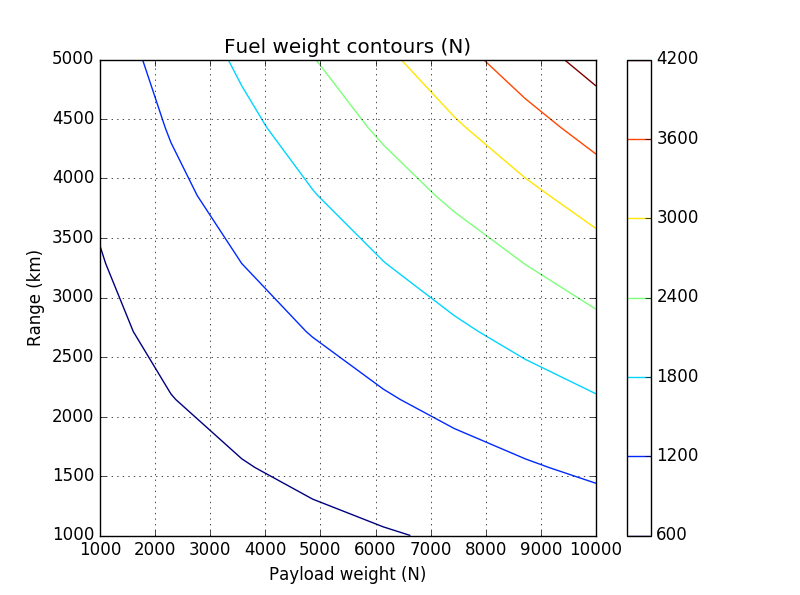
\includegraphics[width=0.9\linewidth]{mission2/W_fcontours.png}
    \end{subfigure}%
    ~
    \begin{subfigure}[t]{0.5\linewidth}
        \centering
        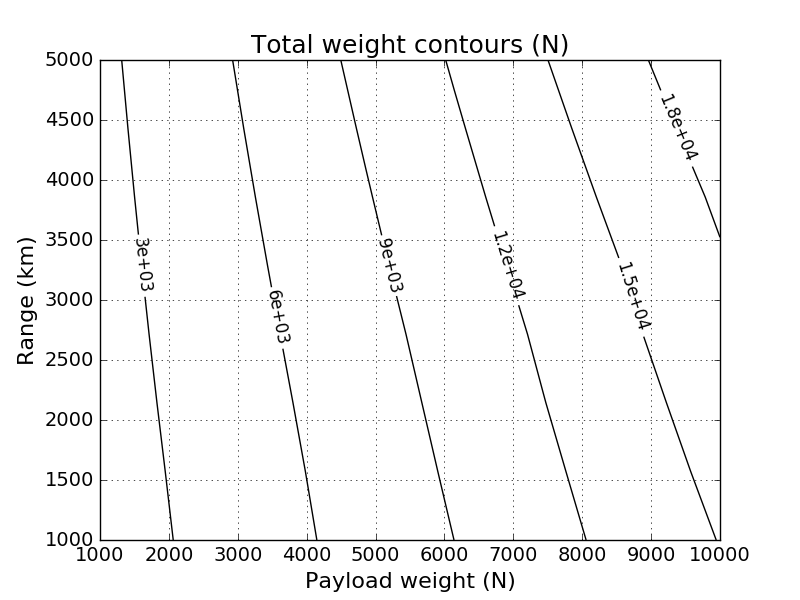
\includegraphics[width=0.9\linewidth]{mission2/Wcontours.png}
    \end{subfigure}
    \caption{The fuel and total weight Pareto frontiers with respect to range and payload inputs.}
    \label{f:pareto}
\end{figure*}

In Section~\ref{s:fuel} we had to weigh whether or not it was worth losing the mathematical
guarantees of convexity to be able to model fuel storage. Now we can use our \gls{SP} model to understand
the tradeoffs in fuel storage, and when it is beneficial to store fuel in the wing versus the fuselage.

\begin{center}
\begin{figure}
    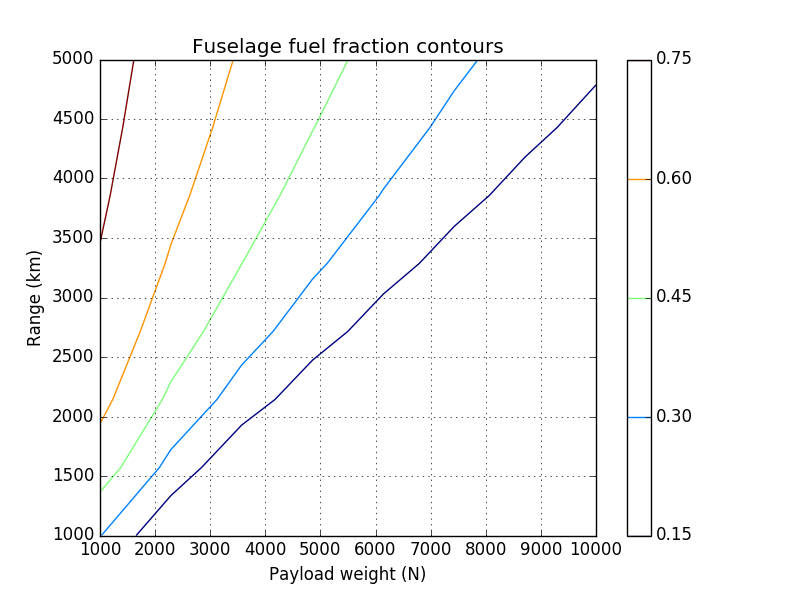
\includegraphics[width=0.45\linewidth]{mission2/FuseFuelFraccontours.png}
    \caption{The lower right of the graph shows where fuel storage in the fuselage is not beneficial.}
    \label{f:fusefuelfrac}
\end{figure}
\end{center}

Figure~\ref{f:fusefuelfrac} shows how designs for different range and payload requirements
allocate fuel differently within the aircraft. As the mission range increases for a given payload weight,
more and more fuel is allocated within the fuselage as a proportion of total fuel. Since fuselage fuel
volume is directly related to increased fuselage drag, it is logical that no fuel is put in the fuselage
until the fuel volume constraint in the wing becomes tight. And this is the behavior that is observed.

\section{Model debugging in mission design}

There are still significant weaknesses in the model that mission design often exploits to arrive at solutions
that do not seem physical. In this specific modeling example, it shows the weaknesses of the engine model.

We can see this through the engine weight contours plots with respect to range and payload as shown in
Figure~\ref{f:wesens}. There is clearly something unphysical or unintuitive happening towards the top
right of the contour plot, where the engine weight goes down even as the range increases for constant payload.

\begin{center}
\begin{figure}
    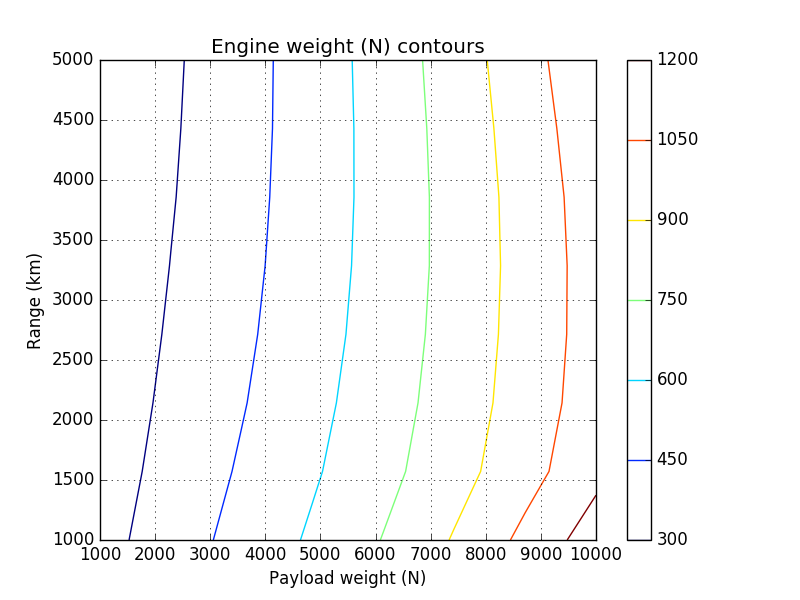
\includegraphics[width=0.45\linewidth]{mission2/W_econtours.png}
    \caption{The engine weight decreases for constant payload towards the right of the graph,
            an unintuitive result.}
    \label{f:wesens}
\end{figure}
\end{center}

The first weakness is the fact that the engine can supply the same amount of power
regardless of altitude. For naturally aspirated piston engines, we would expect the maximum power available to
drop with altitude; adding such a lapse rate will improve how much we trust the engine model.
The second is the lack of an engine \BSFC model. Empirical data shows that the
\BSFC of an engine deteriorates at low power outputs.

This is a key example of how optimization cannot replace engineering intuition. Even though our model
contains many of the key tradeoffs in aircraft design, assumptions can have a significant impact on the
quality of the optima.

In Sections~\ref{s:lapse} and \ref{s:BSFC}, these improvements will be implemented using more data-based modeling.
Then in Section\ref{s:compare},
we can see how improved modeling affects the results of the model.

\subsection{Engine lapse rate model}
\label{s:lapse}

Data-based modeling techniques have been detailed in Section~\ref{s:datafit}, so the author will
not linger here. But much in the same way posynomial fits were created for the relationship between
engine maximum power and weight, the lapse rate of the engine was fitted with respect to throttle level.
This model requires the insertion of another signomial equality into the model. Consider the
posynomial inequality expression below:

\begin{equation}
    \label{e:lapse}
    1 \geq L + \frac{P_{shaft,alt}}{P_{shaft,max}}
\end{equation}

Since the \BSFC of a normally aspirated piston engine would be expected to improve
as the $P_{shaft} \xrightarrow[]{} P_{shaft,alt}$, the maximum shaft
power at altitude has downward pressure on it from the fuel burn objective. This means that the
inequality doesn't adequately lower bound the $P_{shaft,alt}$. If we try to flip the inequality in
Constraint~\ref{e:lapse}, then $P_{shaft,alt}$ is upper-unbounded, so with our current parametrization
of the shaft power, we must use a signomial equality.

\subsection{Making use of sensitivities: engine \BSFC model}
\label{s:BSFC}

The \BSFC is one of the variables that the model is most sensitive to (total sensitivity over all mission segments of 0.59),
and it has yet to be modeled. As
stated in Section~\ref{s:lapse}, the \BSFC of a naturally-aspirated piston engine improves as the engine puts out more power.

BSFC has downward pressure due to the objective function, and therefore must be lower-bounded. This makes
it amenable to multiple-term posynomial fits.

First, a monomial fit of the $\frac{\BSFC}{\BSFC_{min}}$ versus $\frac{P_{shaft}}{P_{shaft,alt}}$ was created.
The result is shown in Figure~\ref{f:P_BSFC}.

\begin{center}
    \begin{figure}
        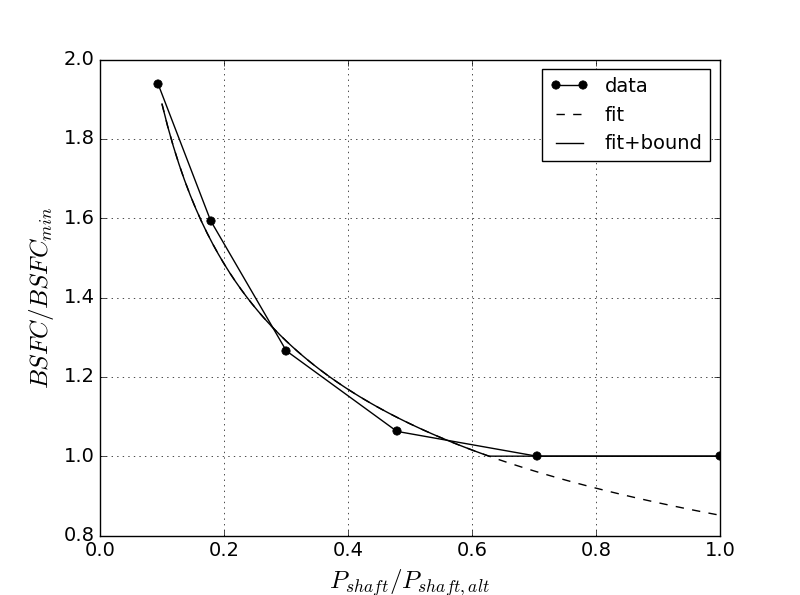
\includegraphics[width=0.5\textwidth]{P_BSFC.png}
        \caption{$\frac{\BSFC}{\BSFC_{min}}$ versus $\frac{P_{shaft}}{P_{shaft,alt}}$ data fit. Note that the fit is
        not able to capture the tail ends of the curve.}
        \label{f:P_BSFC}
    \end{figure}
\end{center}

Although the r.m.s. error of the fit is low (0.015) due to the small number of data points,
there is a significant deterioration in the quality of the
fit as $\frac{P_{shaft}}{P_{shaft,alt}} \xrightarrow[]{} 1$,
and increasing the number of posynomial terms in the fit does not alleviate this problem. It
turns out that fitting with respect to lapse rate using the simple relation $1 = L + \frac{P_{shaft}}{P_{shaft,alt}}$
resolves the issue. The fit with respect to lapse rate, which has been implemented in the model, is
shown in Figure~\ref{f:lapse_BSFC.png}

\begin{center}
    \begin{figure}
        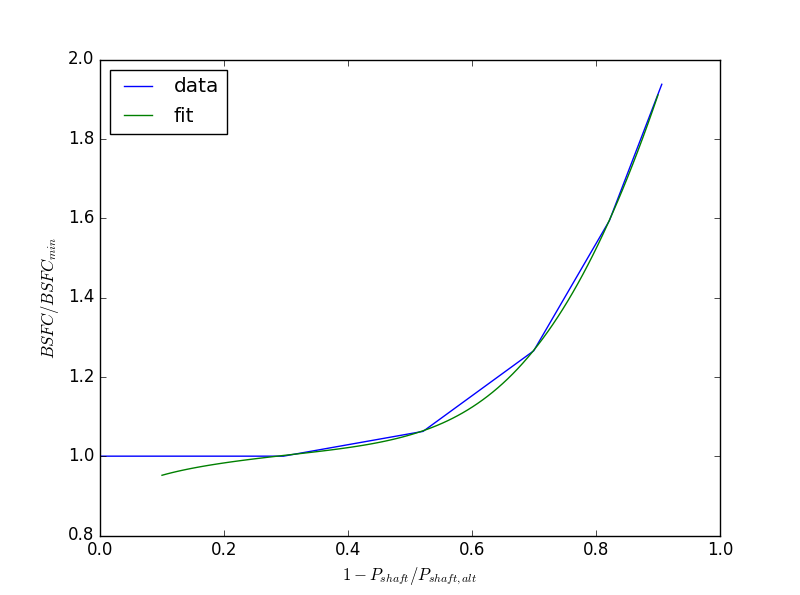
\includegraphics[width=0.5\textwidth]{lapse_BSFC.png}
        \caption{Engine lapse \% $L$ versus $\frac{P_{shaft}}{P_{shaft,alt}}$ data fit. This fit has minimal
        RMS error.}
        \label{f:lapse_BSFC}
    \end{figure}
\end{center}

The r.m.s. error of the new fit is less than $10^{-10}$, since we are able to find a 2-term posynomial that
goes through the seven data points to numerical precision.
The improvement of the fit thanks to a simple variable transformation shows that
parametrization can be important to the level of accuracy and fidelity of a model.

\subsection{Comparing models under different sets of constraints}
\label{s:compare}

We would first like to see that the behavior that doesn't suit our engineering intuition, namely the
decrease in engine weight with increased range, disappear. And this is exactly
what we observe in Figure~\ref{f:wesensimp}.

\begin{center}
\begin{figure}
    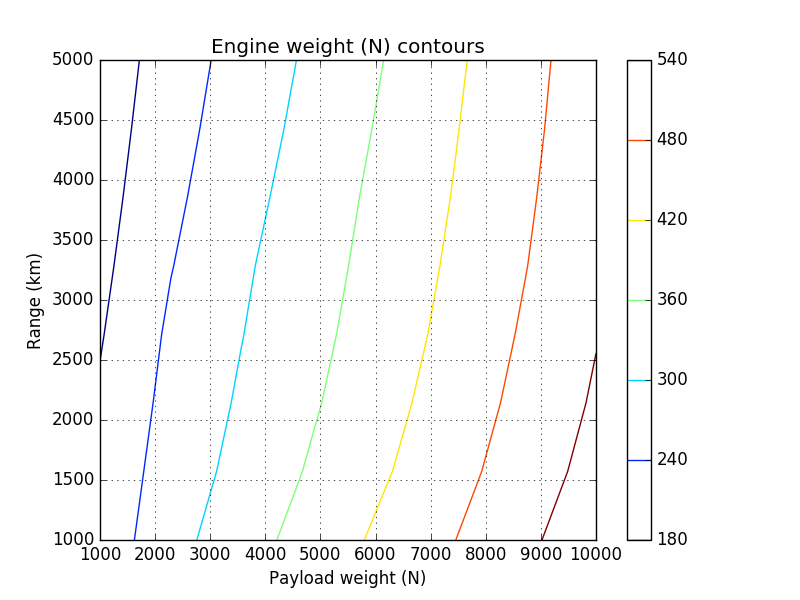
\includegraphics[width=0.45\linewidth]{mission4/W_econtours.png}
    \caption{The engine weight scales appropriately with range and payload with the improved engine model.}
    \label{f:wesensimp}
\end{figure}
\end{center}

The inputs to the mission model, for both the model with and without lapse rate and \BSFC models,
has been detailed in Table~\ref{t:missioninputs}.

\begin{footnotesize}
\begin{center}
\begin{longtable}{llcl}
\toprule
Constants & Value & Units & Description\\ \midrule
$C$ & 120  & $~\mathrm{\tfrac{1}{hr}}$ & hourly cost index \\
$Range$ & 3000  & $~\mathrm{km}$ & aircraft range \\
$T/O factor$ & 2  & $$ & takeoff thrust factor \\
$V_{min}$ & 25  & $~\mathrm{\tfrac{m}{s}}$ & takeoff speed \\
$W_p$ & 6250  & $~\mathrm{N}$ & payload weight \\
$h_{cruise}$ & 5000  & $~\mathrm{m}$ & minimum cruise altitude \\
    \caption{Inputs to the \textbf{\textit{Mission}} model.}
    \label{t:missioninputs}
\end{longtable}
\end{center}
\end{footnotesize}

%TODO: add table comparing the results of the different missions

And most importantly, we should see changes in the sensitivity contours that may (or sometimes may not)
agree with our engineering intuition. This is a valuable feature of optimization coupled in design.

\section{Multimission design}
\label{s:multimission}

Having created a mission profile for the SimPleAC, it only takes one extra level of
hierarchy to do multimission design. Now we vectorize the mission models flown by the same aircraft.

\begin{figure}[!h]
    \centering\small\sffamily
    \begin{forest}
        sn edges,
        l sep+=1em,
        for children={
        l sep+=1em,
        }
        [\textit{\textbf{Multimission}},name=multimission
        [\textit{\textbf{Mission}},name=mission1
        [\textit{\textbf{\shortstack{Aircraft\\Perf.}}},name=ap1[,name=ap1d,edge=dotted]]
        [\textit{\textbf{\shortstack{Aircraft\\Perf.}}},name=ap2[,name=ap2d,edge=dotted]]
        ]
        [[[\textbf{Aircraft},name=ac[,name=acd,edge=dotted]]]]
        [\textit{\textbf{Mission}},name=mission2
        [\textit{\textbf{\shortstack{Aircraft\\Perf.}}},name=ap3
        [,name=ap3d,edge=dotted]]
        [\textit{\textbf{\shortstack{Aircraft\\Perf.}}},name=ap4
        [,name=ap4d,edge=dotted]]
        ]
        ]
        \draw[->] (ac) -- (ap1);
        \draw[->] (ac) -- (ap2);
        \draw[->] (ac) -- (ap3);
        \draw[->] (ac) -- (ap4);
        \draw[->] (ac) -- (mission1);
        \draw[->] (ac) -- (mission2);
        \node[draw,rectangle,fit={(ap1) (ap1d)}] {};
        \node[draw,rectangle,fit={(ap2) (ap2d)}] {};
        \node[draw,rectangle,fit={(ap3) (ap3d)}] {};
        \node[draw,rectangle,fit={(ap4) (ap4d)}] {};
        \node[draw,circle,fit={(mission1) (ap1) (ap2) (ap1d) (ap2d)}] {};
        \node[draw,circle,fit={(mission2) (ap3) (ap4) (ap3d) (ap4d)}] {};
    \end{forest}
    \caption{Multimission uni-directional graph, with $N_{segments} = 2$ and $N_{missions} = 2$.}
    \label{f:multimission}
\end{figure}

Now the vectorization has gone down two levels, where each performance model is vectorized $N_{segments} \times N_{missions}$ times,
and each mission model is vectorized $N_{missions}$ times. The single instance of \textbf{Aircraft}
is passed on as an argument to all of these models, which makes sure that both its
static and performance constraints are satisfied for each flight segment
of every mission.

\subsection{Complex objective functions: behavior in log-space}

The objective function of the \textbf{\textit{Multimission}} model has to be
a posynomial that puts pressure on the variables in every \textbf{\textit{Mission}} model. For example, knowing that
$W_{f_{mission}} \frac{1}{\mathrm{N}} + C \times t_{flight}$ is a valid objective functions to the single mission,
the objective function below for $N_{missions}$

\begin{equation}
    \mathrm{Objective} \geq \sum_{n=1}^{N_{missions}} W_{f_{mission}} \frac{1}{\mathrm{N}} + \mathrm{C} \times t_{flight}
    \label{e:compObj}
\end{equation}

will also work, since the same aircraft will fulfill both missions and are linked.
Assuming that $N_{missions} = 2$, note that an objective of the type below will also work

\begin{equation}
    \mathrm{Objective} \geq W_{f_{mission_{1}}} \frac{1}{\mathrm{N}} + \mathrm{C}_{2} \times t_{flight_{2}}
    \label{e:sepObj}
\end{equation}

but will require some management in variable boundedness since some internal variables,
namely  $W_{f_{mission_{2}}}$ and $t_{flight_{1}}$, will diverge to numerical infinity. Simply upper bounding the variables
internally will resolve boundedness issues. For this kind of objective, the
performance of the aircraft will be a compromise with respect to aircraft optimized purely
for mission time for the first mission or fuel burn for the second mission.

The SimPleAC will be optimized for the 2-mission scenario for both objectives~\ref{e:compObj} and \ref{e:sepObj} and compared against
the single mission solution. The inputs to the model are specified in Table~\ref{t:mminputs}.



\subsection{Potential extensions of multimission design}

Multimission design can

The design of modular systems

Multimission design also allows us to design systems with potential future extensibility. A good example from aircraft design
is the design of a family of aircraft, and more specifically 'stretchable' aircraft. In
this case, we could design a series of aircraft that have aerodynamic surfaces and engines
in common, but have different length fuselages to accommodate different numbers of passengers.


%\chapter{Flexibility and modularity of GPkit models}
\label{ch4:modularity}

In this section, we will abandon the SimPleAC, and move to examine one of the
most sophisticated models and largest models to come out of the \gls{CEG}, SPaircraft.
SPaircraft is a commercial aircraft design tool that makes use of component-
based performance modeling to optimize different configurations of aircraft in
both single- and multi-mission scenarios. This model and its subcomponents will
demonstrate how we can buil

\section{Describing the component-based design framework of SPaircraft}

In a similar fashion to SimPleAC,
SPaircraft has a strict maintenance of variables and constraint hierarchy
as shown in Figure~\ref{forest:SPaircrafttree}, with additional
aircraft components, and
cruise and climb profile classes which differentiate between the different
kinds of flight segments.

\begin{figure}[!h]\centering\small\sffamily
\begin{forest}
        [\textit{\textbf{Mission}}
            [\textit{Atmosphere}]
            [\textit{\textbf{Cruise Profile}},name=Cr]
            [\textit{\textbf{Climb Profile}},name=Cl
                [\textit{\textbf{\shortstack{Aircraft\\Performance}}},name=Ap
                    [\textbf{Aircraft}
                        [\textbf{Wing}]
                        [\textbf{Fuselage}]
                        [\textbf{Engine}]
                        [\textbf{HT}]
                        [\textbf{VT}]
                        [\textbf{Landing Gear}]
                    ]
                    [\textit{\shortstack{Wing\\Perf.}}]
                    [\textit{\shortstack{Fuselage\\Perf.}}]
                    [\textit{\shortstack{Engine\\Perf.}}]
                    [\textit{\shortstack{HT\\Perf.}}]
                    [\textit{\shortstack{VT\\Perf.}}]
               ]
            ]
        ]
    \draw (Cr.south) -- (Ap.north);
    \end{forest}
\caption{Hierarchy of the SPaircraft model. Models that include sizing variables are
bolded while models that include performance variables are italicized. 
There are models that contain both kinds of variables.}
\label{forest:SPaircrafttree}
\end{figure}

\section{Example problem: Creating a modular tail structural model}

\subsection{Horizontal Tail Terminology}
\begin{tabbing}
$I_{\rm{cap}}$ = non-dimensional spar cap area moment of inertia \\
$L_{\rm{ht}}$ = horizontal tail downforce \\
$L_{\rm{ht}_{\rm{max}}}$ = maximum horizontal tail downforce \\
$L_{\rm{ht}_{rect}}$ = rectangular horizontal tail load \\
$L_{\rm{ht}_{\rm{rect}_{\rm{out}}}}$ = rectangular horizontal tail load outboard\\
$L_{\rm{ht}_{\rm{tri}}}$ = triangular horizontal tail load \\
$L_{\rm{ht}_{tri_{\rm{out}}}}$ = triangular horizontal tail load outboard\\
$L_{\rm{shear}}$ = maximum shear load at pin-joint\\
$M_{\rm{r}}$ = moment per chord at horizontal tail root \\
$M_{\rm{r}_{\rm{out}}}$ = moment per chord at pin-joint\\
$N_{\rm{lift}}$ = horizontal tail loading multiplier \\
$S_{\rm{ht}}$ = horizontal tail area \\
$W_{\rm{cap}}$ = weight of spar caps \\
$W_{\rm{struct}}$ = horizontal tail wingbox weight \\
$W_{\rm{web}}$ = weight of shear web \\
$\lambda_{\rm{ht}}$ = horizontal tail taper ratio \\
$\nu$ = dummy variable = $(t^2 + t + 1)/(t+1)^2$ \\
$\pi_{\rm{M-fac}}$ = pi-tail bending structural factor \\
$\rho_{\rm{cap}}$ = density of spar cap material \\
$\rho_{\rm{web}}$ = density of shear web material \\
$\sigma_{max,shear}$ = allowable shear stress \\
$\sigma_{\rm{max}}$ = allowable tensile stress \\
$\tau_{\rm{ht}}$ = horizontal tail thickness/chord ratio \\
$b_{\rm{ht}}$ = horizontal tail span \\
$b_{\rm{ht}_{\rm{out}}}$ = horizontal tail outboard half-span\\
$c_{\rm{attach}}$ = horizontal tail chord at the pin-joint \\
$c_{\rm{root}_{\rm{ht}}}$ = horizontal tail root chord \\
$c_{\rm{tip}_{\rm{ht}}}$ = horizontal tail tip chord \\
$g$ = gravitational acceleration \\
$q_{\rm{ht}}$ = substituted variable = 1 + taper \\
$r_h$ = fractional wing thickness at spar web \\
$t_{\rm{cap}}$ = non-dim. spar cap thickness \\
$t_{\rm{web}}$ = non-dim. shear web thickness \\
$w$ = wingbox width-to-chord ratio \\
$w_{\textrm{fuse}}$ = fuselage half-width \\
\end{tabbing}

\subsection{Conventional horizontal tail model}

Consider the set of equations considered in \cite{SP_ac_design} to size
the structure of a conventional horizontal tail. 

\begin{align}
\label{e:HTorig}
\begin{split}
    0.92 w\tau_{\rm{ht}} t_{\rm{cap}}^2 + I_{\rm{cap}} &\leq \frac{0.92^2}{2}w\tau_{\rm{ht}}^2t_{\rm{cap}}\\
    8 &\geq N_{\rm{lift}}M_{\rm{r}}(\AR_{\rm{ht}})q_{\rm{ht}}^2\frac{\tau_{\rm{ht}}}{S_{\rm{ht}} I_{\rm{cap}}\sigma_{\rm{max}}}\\
    12 &\geq \frac{L_{\rm{max}} N_{\rm{lift}} q^2}{\tau_{\rm{ht}} S t_{\rm{web}} \sigma_{\rm{max-shear}}}
\end{split}
\end{align}

Now, using a set of variables that includes the original parametrization of the wing, 
we would like to extend this structural model to be able to design a pi horizontal tail
with the same loading as well as a conventional horizontal tail. Pi tails are prominently
featured in the D8 configuration shown in Figure~\ref{f:D8}, and so it is important to
be able to capture the structural benefits of a pi horizontal tail versus a conventional
horizontal tail when designing a D8.

\begin{figure*}[t!]
    \centering
    \begin{subfigure}[t]{0.5\linewidth}
        \centering
        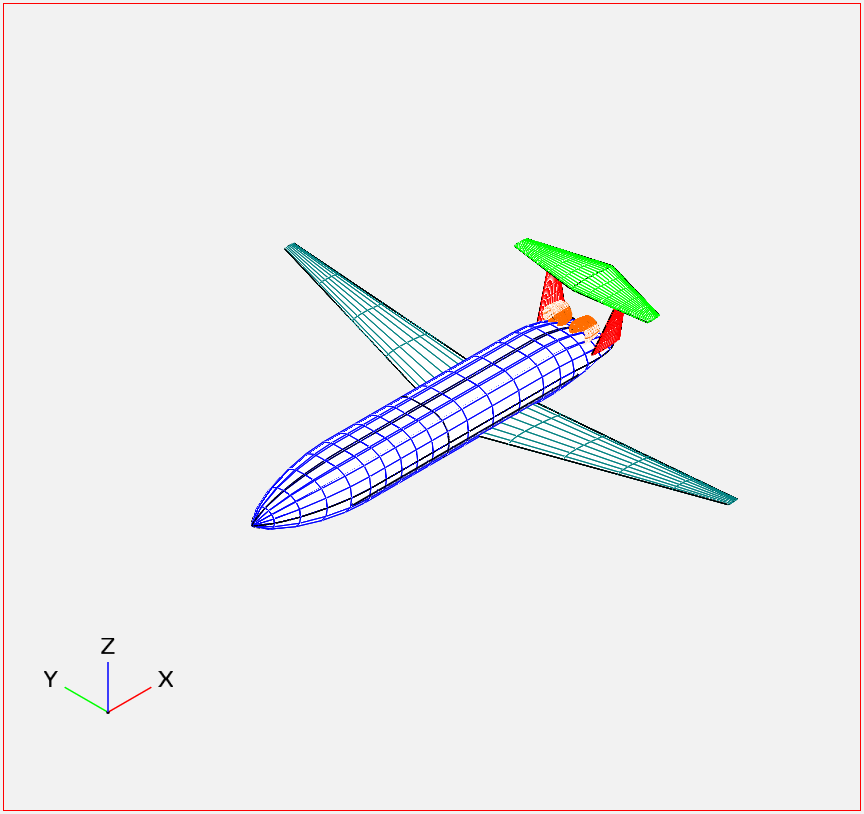
\includegraphics[width=0.75\linewidth]{optimal_D8-1.png}
        \caption{Isometric view}
    \end{subfigure}%
    ~
    \begin{subfigure}[t]{0.5\linewidth}
        \centering
        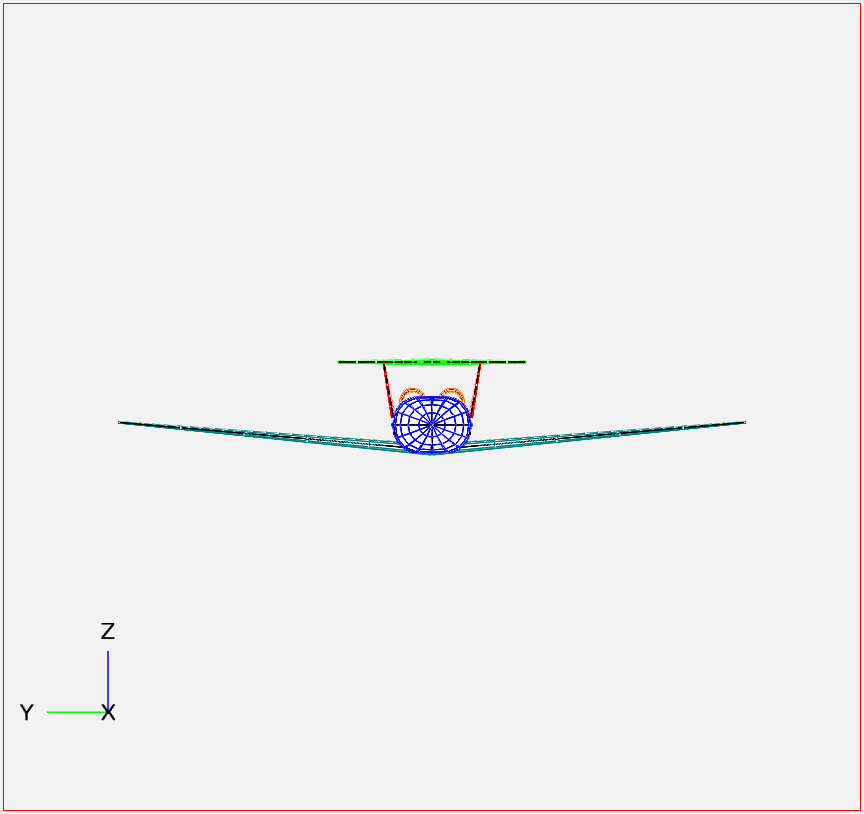
\includegraphics[width=0.75\linewidth]{optimal_D8-3.png}
        \caption{Front view}
    \end{subfigure}
    \caption{The pi tail is prominently featured in the D8 configuration, with engines
    embedded between the vertical tails.}
    \label{f:D8}
\end{figure*}

This section will derive a new set of constraints, which are compatible with 
both conventional tail and pi-tail architectures, and in the process demonstrate the
capabilities of \gls{GP} in making modular component models.

\subsection{Assumptions}

We have to make assumptions about the structure of the problem to be able
to determine the loading on the horizontal tail. This can be quite the chicken-and-egg problem
and it is often not clear how to proceed. It requires engineering understanding
from the designer, which we consider to be key in \gls{GP} based design. But here is an
intuitive description of the approach for the current example. 

Note that in our derivation we would like to err on the side of conservatism always, since we would
rather be in a more restricted and realistic subset of the design space, rather than 
expanding our feasible set to include solutions that are optimistic and potentially
infeasible. The assumptions for the derivation are as follows:

\begin{enumerate}
    \item \textbf{The lift per unit span is proportional to local chord.} This allows 
    us to neglect the effects of lift rolloff towards the wingtips, which is difficult
    to model in a \gls{GP} framework, and allows us to have a lift distribution to base
    our structural model on.  Since the horizontal tail model will
    be more heavily loaded towards its wingtips than an actual tail, the loads
    on the tail model are conservative. 
    \item \textbf{The horizontal tail has a constant taper ratio.} We would like to 
    capture the effects of geometry on the problem with a good 
    accuracy, but without making the physical relations unwieldy.
    This basic parametrization
    gives a good representation of the horizontal tail planform.  
    Constant taper tail sections are observed in real aircraft, and
    higher degrees of freedom in horizontal tail chord are considered unnecessary
    at this level of fidelity.
    \item \textbf{The horizontal and vertical tail joint is a fuselage width away from 
    the centerline of the aircraft.} In the pi-tail configuration the vertical tails are 
    often canted outward for aerodynamic benefits. However, we would like to avoid making 
    assumptions about this, and make the conservative approximation that the vertical tails
    are perfectly vertical, and join the fuselage and the horizontal tail at $w_{fuse}$, the
    width of the fuselage.
    \item \textbf{The horizontal and vertical tail interface is a pin joint.} This implies 
    that the joint does not exert a moment on the horizontal tail, and a conservative 
    assumption from an engineering perspective. We do not want to expose such a fine 
    interface to moments that may cause failure. \label{item:pinjoint}
    \item \textbf{The shear and moment distributions on the horizontal tail are 
    linearized.} The reasons for this assumption will become more clear in 
    the following sections. 
\end{enumerate}

\subsection{Loads on a horizontal tail}
\label{s:HTloads}

As with a majority of \gls{GP} formulations, we have to consider the fundamental physics to 
be able to derive a new set of constraints. This requires the examination of free body
diagrams.

\subsubsection{Sample Free Body Diagram and Load Distributions}
\label{s:loadDistributions}

With the aforementioned assumptions, the notional free body diagram diagram of the
pi-tail is shown at the top of Figure~\ref{f:HTFBD}.

\begin{figure}[!ht]
\centering
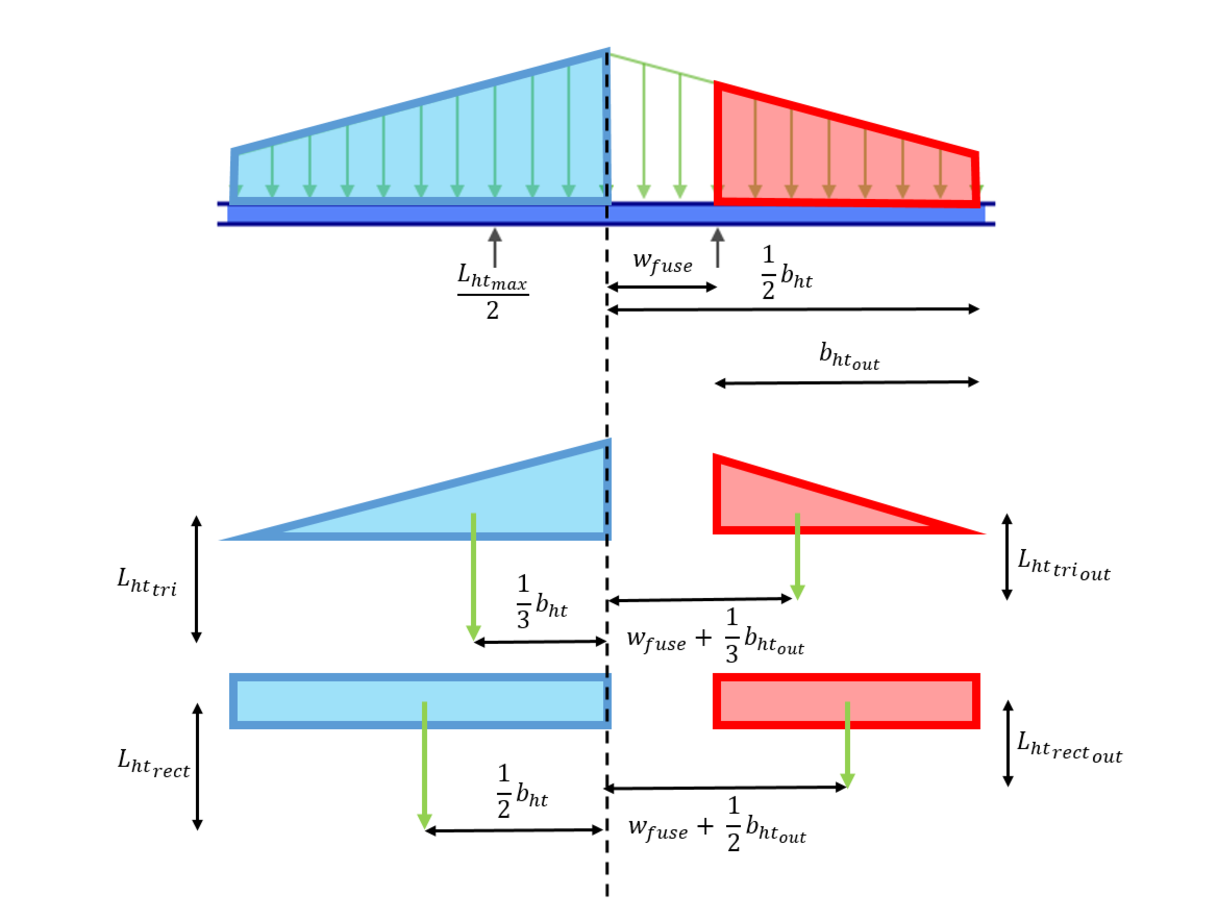
\includegraphics[width=.8\textwidth]{HTFBD.pdf}
\caption{Free body diagram of the forces on the horizontal tail. The distributed 
lift force, which is assumed to be proportional to local chord, is partitioned 
into triangular and rectangular components.}
\label{f:HTFBD}
\end{figure}

The free body diagrams from Figure~\ref{f:HTFBD} result in the
shear and moment distributions presented in Figures~\ref{f:HTshear} and
\ref{f:HTmoment} respectively. The diagrams include both the distributed lift
loads (green arrows in Figure \ref{f:HTFBD}) and the point loads of imposed on
the pin joints by the vertical tails. These diagrams allow
us to make several important observations.


\begin{figure}[!ht]
    \centering
    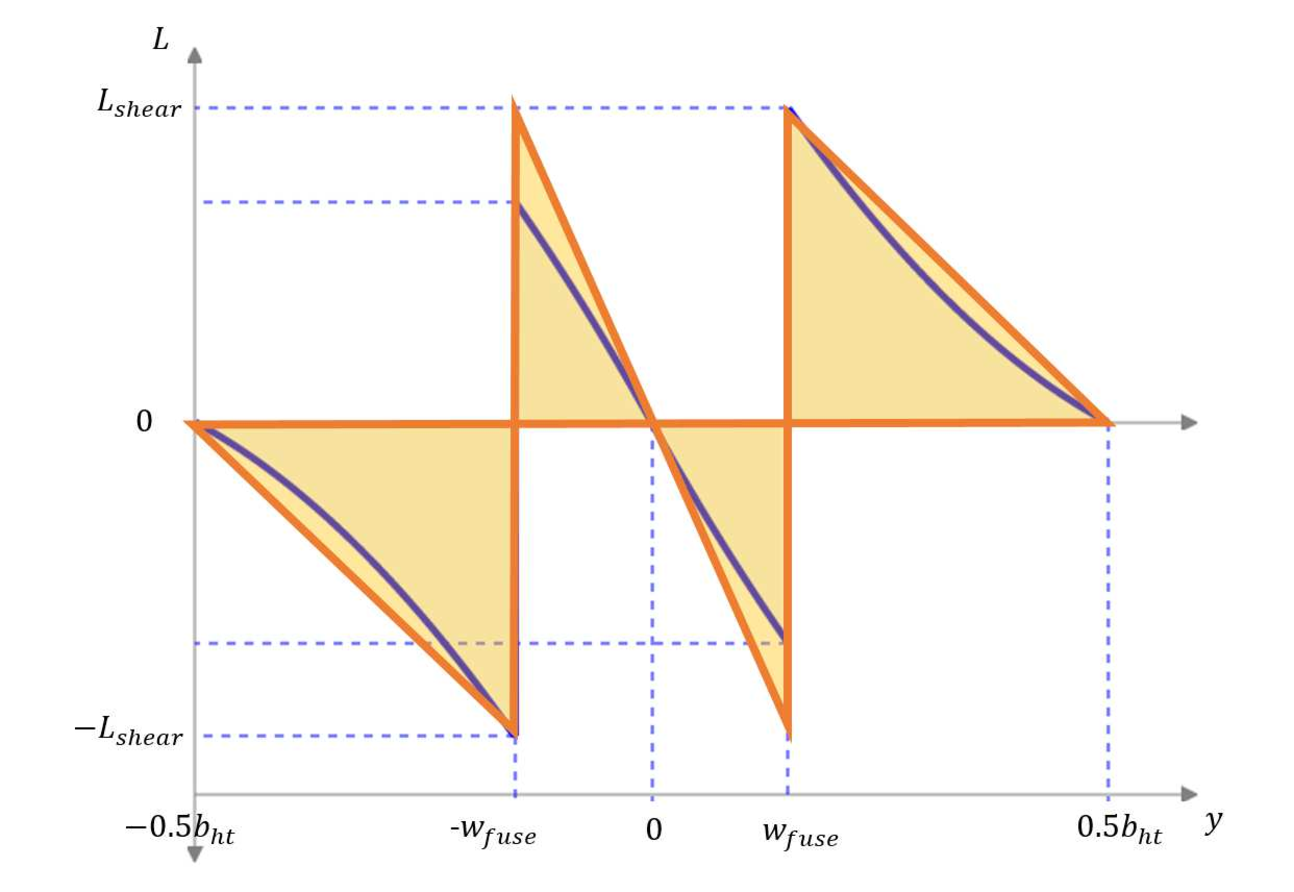
\includegraphics[width = 0.7\linewidth]{HTshear.pdf}
    \caption{Shear diagram of the pi-tail. The blue line shows the actual 
loading, while the yellow line with infill shows the assumed load distribution.}
    \label{f:HTshear}
\end{figure}

\begin{figure}[!ht]
    \centering
    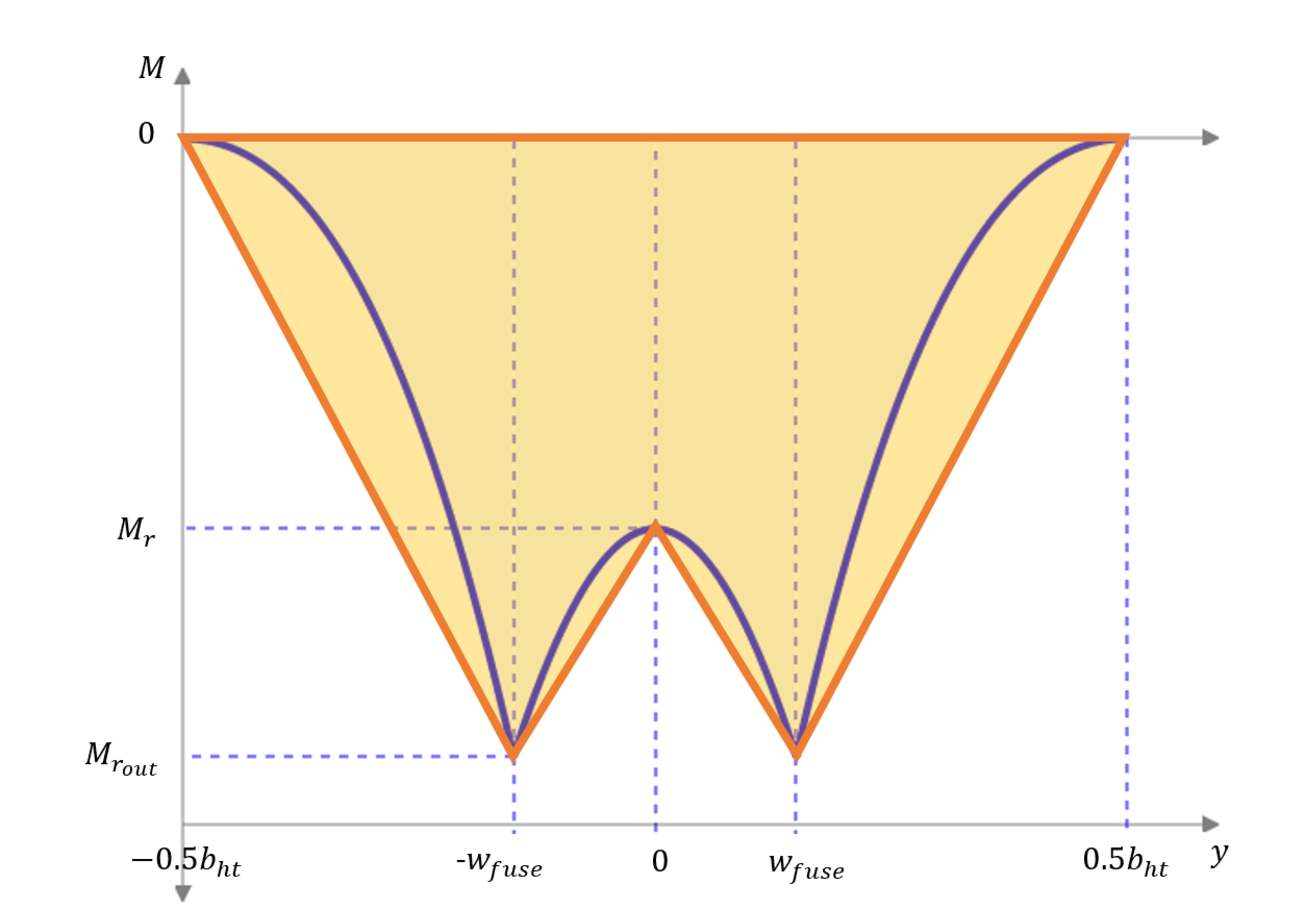
\includegraphics[width = 0.7\linewidth]{HTmoment.pdf}
    \caption{Moment diagram of the pi-tail. The blue line shows the actual 
loading, and the yellow line shows the assumed load distribution}
    \label{f:HTmoment}
\end{figure}

The first is that the pi horizontal tail becomes a conventional tail in
the limit where $w_{fuse} \xrightarrow[]{} 0$. This gives us the clue that we can
have a model that can accurately represent the structural constraints on both kinds
of tails. Furthermore, in the limit, we can confirm that the new structural model
arrives at the same solution as the original structural model, helping us debug
potential issues in the transition.

Another important feature of the load distributions that they can be represented
with relatively high accuracy using a linearization of the load distributions,
an approximation that is strictly conservative.
The yellow-outlined load distributions in Figures~\ref{f:HTshear} and \ref{f:HTmoment}
show how the loads are approximated
in this case. The linear approximation will help us in leveraging Equations
~\ref{e:HTorig} to size both horizontal tail configurations.

As a note, the pin-joint assumption ensures the vertical tail structural constraints do not
need to be modified for the pi-tail configuration. 

\subsubsection{Load Derivation}

In Figure~\ref{f:HTFBD}, we have subdivided the constant taper horizontal tail into its
rectangular (no taper) and triangular (fully tapered) components. Using the assumption
that the lift per unit length is proportional to the local chord, we can define
$L_{\rm{ht}_{rect}}$ and $L_{\rm{ht}_{\rm{tri}}}$
to be half the lift generated by the rectangular and triangular
sections of the wing (the blue rectangle and triangle in Figure~\ref{f:HTFBD}) respectively.

\begin{align}
    L_{\rm{ht}_{rect}} &\geq \frac{L_{\rm{ht}_{\rm{max}}} c_{\rm{tip}_{\rm{ht}}} b_{\rm{ht}}}{2 S_{\rm{ht}}}
    L_{\rm{ht}_{\rm{\rm{tri}}}} &\geq \frac{L_{\rm{ht}_{\rm{max}}} (1 - \lambda_{\rm{ht}}) c_{\rm{root}_{\rm{ht}}} b_{\rm{ht}}}{4
S_{\rm{ht}}}
\end{align}
 
After defining the horizontal tail half-span outboard of the pin joint 
($b_{\rm{ht}_{\rm{out}}}$) in a signomial constraint,
the outboard components of the lift loads can be computed
with respect to $L_{\rm{ht}_{rect}}$ and $L_{\rm{ht}_{\rm{tri}}}$. The outboard loads are shown 
in red in Figure~\ref{f:HTFBD}.
 
 \begin{align}
     b_{\rm{ht}_{\rm{out}}} &\geq 0.5b_{\rm{ht}} - w_{\textrm{fuse}}\\
     L_{\rm{ht}_{tri_{\rm{out}}}} &\geq L_{\rm{ht}_{\rm{tri}}} \frac{b_{\rm{ht}_{\rm{out}}}}{(0.5b_{\rm{ht}})^2}\\
     L_{\rm{ht}_{\rm{rect}_{\rm{out}}}} &\geq L_{\rm{ht}_{rect}} \frac{b_{\rm{ht}_{\rm{out}}}}{0.5b_{\rm{ht}}}
 \end{align}
 
The horizontal-vertical tail pin joint is assumed to be exactly at $w_{\textrm{fuse}}$. 
This is a conservative estimate. In most pi-tail configurations the vertical 
tails are canted outwards. The local chord at the pin joint can then be constrained with
the following monomial equality.
 
\begin{equation}
    c_{\rm{attach}} = \frac{b_{\rm{ht}} \lambda_{\rm{ht}} c_{\rm{root}_{\rm{ht}}}}{2 w_{\textrm{fuse}}}
\end{equation}

We have now fully constrained the geometry of the horizontal tail, but
what is required for structural sizing is the bending moment and shear loads.
The maximum moment at the joint is determined by summing the bending moment 
contributions from loads outboard of the joint. 
\begin{equation}
M_{\rm{r}_{\rm{out}}} c_{\rm{attach}} \geq 
                    L_{\rm{ht}_{\rm{rect}_{\rm{out}}}} \frac{1}{2}b_{\rm{ht}_{\rm{out}}} + 
L_{\rm{ht}_{tri_{\rm{out}}}} \frac{1}{3}b_{\rm{ht}_{\rm{out}}},
\end{equation}
 
The maximum shear at the joint is the sum of the outboard shear loads. The 
maximum root moment is the sum of the bending loads from lift and the pin-joint 
load. 
 
\begin{align}
L_{\rm{shear}} &\geq L_{\rm{ht}_{\rm{rect}_{\rm{out}}}} + L_{\rm{ht}_{tri{\rm{out}}}}\\
M_{\rm{r}} c_{\rm{root}_{\rm{ht}}} &\geq L_{\rm{ht}_{\rm{rect}}} \frac{1}{4}b_{\rm{ht}} + L_{\rm{ht}_{\rm{\rm{tri}}}} 
\frac{1}{6}b_{\rm{ht}}  - \frac{1}{2}L_{\rm{ht}_{\rm{max}}} w_{\textrm{fuse}} 
\end{align}

Finally, the wingtip moment is set equal to zero with a signomial equality 
constraint to satisfy the zero-moment condition on the pin joint. This is one
of the few cases where a signomial equality is required, since the pressures
on the wing can change the favored direction of the GP-compatible inequality depending on
the aircraft configuration.

\begin{equation}
    \frac{b_{\rm{ht}}}{4} L_{\rm{ht}_{\rm{rect}}} + \frac{b_{\rm{ht}}}{3} L_{\rm{ht}_{\rm{\rm{tri}}}} = b_{\rm{ht}_{\rm{out}}} 
\frac{L_{\rm{ht}_{\rm{max}}}}{2}
\end{equation}

\subsubsection{Structural Sizing}

Now we adapt the equations from \cite{gp_ac_design} for wing structural sizing using
a linearization of the moment and shear load distributions from Section~\ref{s:HTloads}. The
constraints can be applied to both conventional and pi-tails.

\begin{align}
    0.92 w\tau_{\rm{ht}} t_{\rm{cap}}^2 + I_{\rm{cap}} &\leq \frac{0.92^2}{2}w\tau_{\rm{ht}}^2t_{\rm{cap}}\\
    8 &\geq N_{\rm{lift}}M_{\rm{r}_{\rm{out}}}(\AR_{\rm{ht}})q_{\rm{ht}}^2\frac{\tau_{\rm{ht}}}{S_{\rm{ht}} I_{\rm{cap}}\sigma_{\rm{max}}}\\
    12 &\geq \frac{2L_{\rm{shear}} N_{\rm{lift}} q^2}{\tau_{\rm{ht}} S t_{\rm{web}} \sigma_{\rm{max-shear}}}
\end{align}

The changes to the model in \cite{gp_ac_design} are:
\begin{itemize}
    \item In the shear constraint replacing $L_{\rm{ht}_{\rm{max}}}$ with $2L_{\rm{shear}}$. 
This is done because the shear loads for the pi-tail are different than the 
maximum lift loads for the conventional tail. 
    \item Replacing $M_{\rm{r}}$ with $M_{\rm{r}_{\rm{out}}}$, the moment per unit chord at the 
pin joint. For a pi-tail, maximum bending loads occur at the pin joint.
    %, and along with the root moment per unit chord $M_{\rm{r}}$ can be used to give a 
    %conservative approximation for the mass of the horizontal tail. 
\end{itemize}

The linearization of the shear and bending load distributions simplifies the 
derivation of the structural web and cap weights. Shear web sizing relies on the 
assumption that the maximum shear ($L_{\rm{shear}}$) occurs at the pin-joint and the 
weight of the shear web of the pi-tail under $L_{\rm{shear}}$ is equal to the shear 
web weight of a conventional tail subjected to the the same maximum shear load 
at its root. This is a conservative approximation, the load distribution implied 
by this assumption (shown in yellow in Figure~\ref{f:HTshear}) has a larger
internal area than the actual load distribution. Intuitively, the $L_{\rm{shear}}$ 
for a pi-tail is strictly smaller than the $L_{\rm{shear}}$ a conventional tail of 
the same size and loading. The pi-tail more efficient in shear.

The cap weight of the pi-tail is determined by scaling the cap weight of a 
conventional tail with the same geometry as the pi-tail and a root moment of 
$M_{\rm{r}_{\rm{out}}} c_{\rm{attach}}$. The scaling factor, $\pi_{\rm{M-fac}}$, is the ratio of the 
total shaded bending moment area in Figure~\ref{f:HTmoment} to the sum of the
outboard shaded areas multiplied by the ratio of the outboard half-span to the 
total half-span.

\begin{equation}
    \pi_{\rm{M-fac}} \geq \left[\frac{\frac{1}{2}(M_{\rm{r}_{\rm{out}}} c_{\rm{attach}} +
    M_{\rm{r}} c_{\rm{root}_{\rm{ht}}}) w_{\textrm{fuse}}} {\frac{1}{2}M_{\rm{r}_{\rm{out}}} c_{\rm{attach}} 
b_{\rm{ht}_{\rm{out}}}} + 1.0\right]
    \frac{b_{\rm{ht}_{\rm{out}}}} {0.5b_{\rm{ht}}},
\end{equation}

Given the calculated loads and structural factors, the bending material and 
shear web weight can be calculated. 

\begin{align}
    W_{\rm{cap}} &\geq \frac{\pi_{\rm{M-fac}} 8 \rho_{\rm{cap}} g w t_{\rm{cap}} S_{\rm{ht}}^1.5 \nu}
    {3\AR_{\rm{ht}}^{0.5}}\\
    W_{\rm{web}} &\geq \frac{8 \rho_{\rm{web}} g r_h \tau_{\rm{ht}} t_{\rm{web}} S_{\rm{ht}}^{1.5} 
\nu}{3\AR_{\rm{ht}}^{0.5}}\\
    W_{\rm{struct}} &\geq W_{\rm{web}} + W_{\rm{cap}}
\end{align}

The value for $t_{\rm{cap}}$ is notional in the derivation above. Rather than being 
the spar cap thickness of a pi-tail, it is the spar cap thickness required for a 
conventional tail of the same geometry and a root moment  ($M_{\rm{r}_{\rm{out}}} 
c_{\rm{attach}}$) as a pi-tail. With a similar reasoning as for the shear loads, 
$\pi_{\rm{M-fac}} t_{\rm{cap}}$ for a pi-tail is strictly smaller than the $t_{\rm{cap}}$ for a 
conventional tail of the same geometry and loading, making the pi-tail more 
efficient in bending than a traditional tail. 

\chapter{Conclusion}
\label{ch5:conclusion}

%TODO: much to do here...
TO BE COMPLETED.

This thesis serves to demonstrate methods in \gls{GP} modeling and optimization
rather than provide interesting results, so I will

In Chapter~\ref{ch2:inequalities},

I have defined an aircraft model to show the intuitive nature of \gls{GP}
compatible constraints, and demonstrated how to model a complex
starting from scratch

I concluded with describing the use cases for signomial equalities.

In Chapter~\ref{ch3:extensibility}, I have first presented an intuitive
way to analyze the solution of the \gls{GP}, and draw maximal engineering
understanding from it. I have expanded upon the SimPleAC engine model
in response to the sensitivity information to improve its fidelity,
and modularized it into both component models, and performance and static models.


%In Chapter~\ref{ch4:modularity}, I have presented SPaircraft, one of the more
%advanced \gls{SP} models made in GPkit. I have demonstrated how to model
%a complex component such as the horizontal tail within the GP framework,
%while making it compatible with different potential tail configurations.

\appendix
\chapter{Mathematical Framework}

\section[Geometric Programming]{Geometric Programming\footnote{This section has been borrowed from the paper
titled \textit{Efficient Aircraft Multidisciplinary Design Optimization and Sensitivity Analysis via Signomial Programming},
by Martin York, Berk Ozturk, Edward Burnell and Warren Hoburg.
The paper is undergoing review for publication in the AIAA Journal as of January 24th, 2018.}}
\label{a:gpintro}

Introduced in 1967 by Duffin et al.~\cite{duffingp}, a geometric program \gls{GP} is
a type of constrained optimization problem that becomes convex after a
logarithmic change of variables. Modern interior point methods allow a typical
sparse \gls{GP} with tens of thousands of decision variables and tens of thousands of
constraints to be solved in minutes on a desktop computer~\cite{convex}. These
solvers do not require an initial guess, and guarantee convergence to a
\textit{global} optimum, assuming a feasible solution exists. If a feasible
solution does not exist, the solver will return a certificate of infeasibility.
These impressive properties arise because a GP's objective and
constraints consist of only monomial and posynomial functions, which can be
transformed into convex functions in log space.

A monomial is a function of the form
\begin{equation}\label{e:monomial}
m(\mathbf{u}) = c\prod_{j=1}^{n} u_{j}^{a_{j}}
\end{equation}
where $a_{j} \in \mathbb{R}, c \in \mathbb{R}_{++}$ and $u_{j} \in
\mathbb{R_{++}}$. An example of a monomial is the common expression for lift,
$\frac{1}{2} \rho V^2C_{L}S$. In this case, $\mathbf{u} = (\rho, V, C_{L}, S)$,
$c= 1/2$, and $a = (1, 2, 1, 1)$.

A posynomial is a function of the form
\begin{equation}\label{e:posynomial}
p(\mathbf{u}) = \sum_{k=1}^{K}c_{k}\prod_{j=1}^{n} u_{j}^{a_{jk}}
\end{equation}
where $a_{jk} \in \mathbb{R}, c_{k} \in \mathbb{R}_{++}$ and $u_{j} \in
\mathbb{R_{++}}$. A posynomial is a sum of monomials. Therefore, all monomials
are also one-term posynomials.

A GP minimizes a posynomial objective function subject to monomial equality and
posynomial inequality constraints. A GP written in standard form is

\begin{equation}
\label{e:standardform}
\begin{aligned}
\text{minimize }p_{0}(\mathbf{u})& \\
\text{subject to }p_{i}(\mathbf{u})& \leq 1, i = 1, ...., n_{p}, \\
m_{i}(\mathbf{u})& = 1, i = 1, ..., n_{m}
\end{aligned}
\end{equation}

where $p_{i}$ are posynomial functions, $m_{i}$ are monomial functions, and
$\mathbf{u} \in \mathbb{R}^n_{++}$ are the decision variables. Once a problem
has been formulated in the standard form (Equation \ref{e:standardform}), it can
be solved efficiently.

\section[Signomial Programming]{Signomial Programming\footnote{This section has been borrowed from the paper
titled \textit{Efficient Aircraft Multidisciplinary Design Optimization and Sensitivity Analysis via Signomial Programming},
by Martin York, Berk Ozturk, Edward Burnell and Warren Hoburg.
The paper is undergoing review for publication in the AIAA Journal as of January 24th, 2018.}}
\label{a:spintro}

It is not always possible to formulate a design problem as a GP. This motivates
the introduction of signomials. Signomials have the same form as posynomials
\begin{equation}\label{e:signomial}
s(\mathbf{u}) = \sum_{k=1}^{K}c_{k}\prod_{j=1}^{n} u_{j}^{a_{jk}}
\end{equation}

but the coefficients, $c_{k} \in \mathbb{R}$, can now be any (including
non-positive) real numbers.

A signomial program (SP) is a generalization of GP where the inequality
constraints can be composed of signomial constraints of the form $s(u) \leq 0$..
The log transform of an SP is not a convex optimization problem, but is a
difference of convex optimization problem that can be written in log-space as

\begin{equation}
\begin{aligned}
\text{minimize }f_{0}(\mathbf{x})& \\
\text{subject to }f_{i}(\mathbf{x}) -  g_{i}(\mathbf{x})& \leq 0, i = 1, ...., m
\\
\end{aligned}
\end{equation}

where $f_{i}$ and $g_{i}$ are convex.

There are multiple algorithms that reliably solve signomial programs to
\textit{local} optima~\cite{gpintro, spsolutions}. A common solution heuristic,
referred to as difference of convex programming or the convex-concave procedure,
involves solving a sequence of GPs, where each GP is a local approximation to
the SP, until convergence occurs. It is worth noting that the introduction of
even a single signomial constraint to any GP turns the GP into a \gls{SP}, thus losing
the guarantee of solution convergence to a global optimum. Despite the
possibility of convergence to a local, not global, optimum, SPs are a powerful
tool. The convex approximation, $\hat{f}(x)$, to the non-convex signomial in
log-space, $f(x) - g(x)$, is constructed such that it always satisfies

\begin{equation}
\hat{f}(x) \geq f(x) - g(x) \quad \forall \quad x
\end{equation}

In other words, for each constraint, the feasible set of the convex
approximation $\hat{f}(x) \leq 0$ is a subset of the original SP's feasible set,
$f(x) - g(x) \leq 0$. This means SP inequalities do not require a trust region,
removing the need for trust region parameter tuning and making solving SPs
substantially more reliable than solving general nonlinear programs. Figure
\ref{f:GPapproxs}, where a series of convex (GP compatible) constraints
approximates a non-convex parabolic drag polar in log space, illustrates this
property.

\begin{figure*}[t!]
    \centering
    \begin{subfigure}[t]{0.5\linewidth}
        \centering
        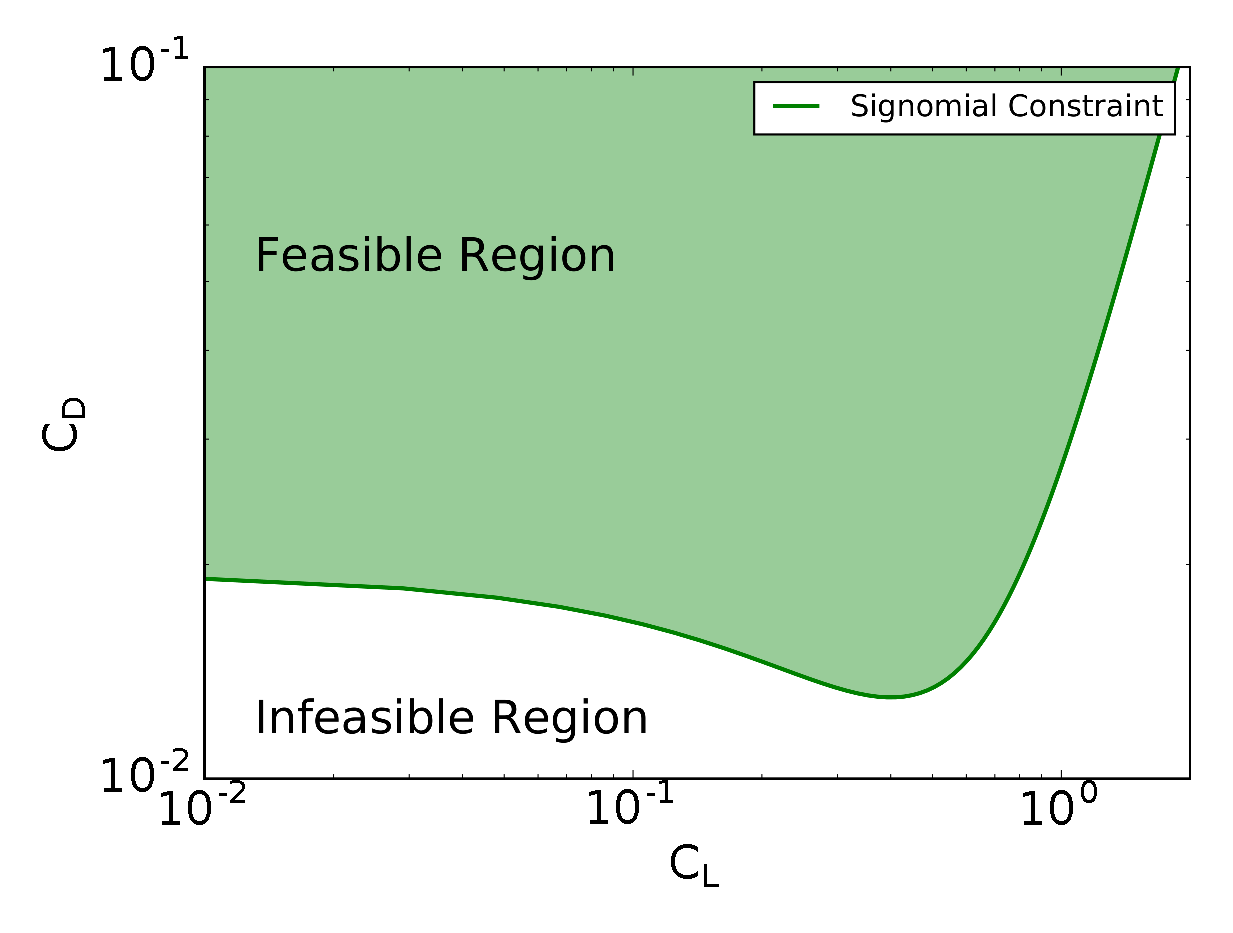
\includegraphics[width=0.9\linewidth]{posyapprox0.eps}
        \caption{Non-convex signomial inequality drag constraint}
    \end{subfigure}%
    ~
    \begin{subfigure}[t]{0.5\linewidth}
        \centering
        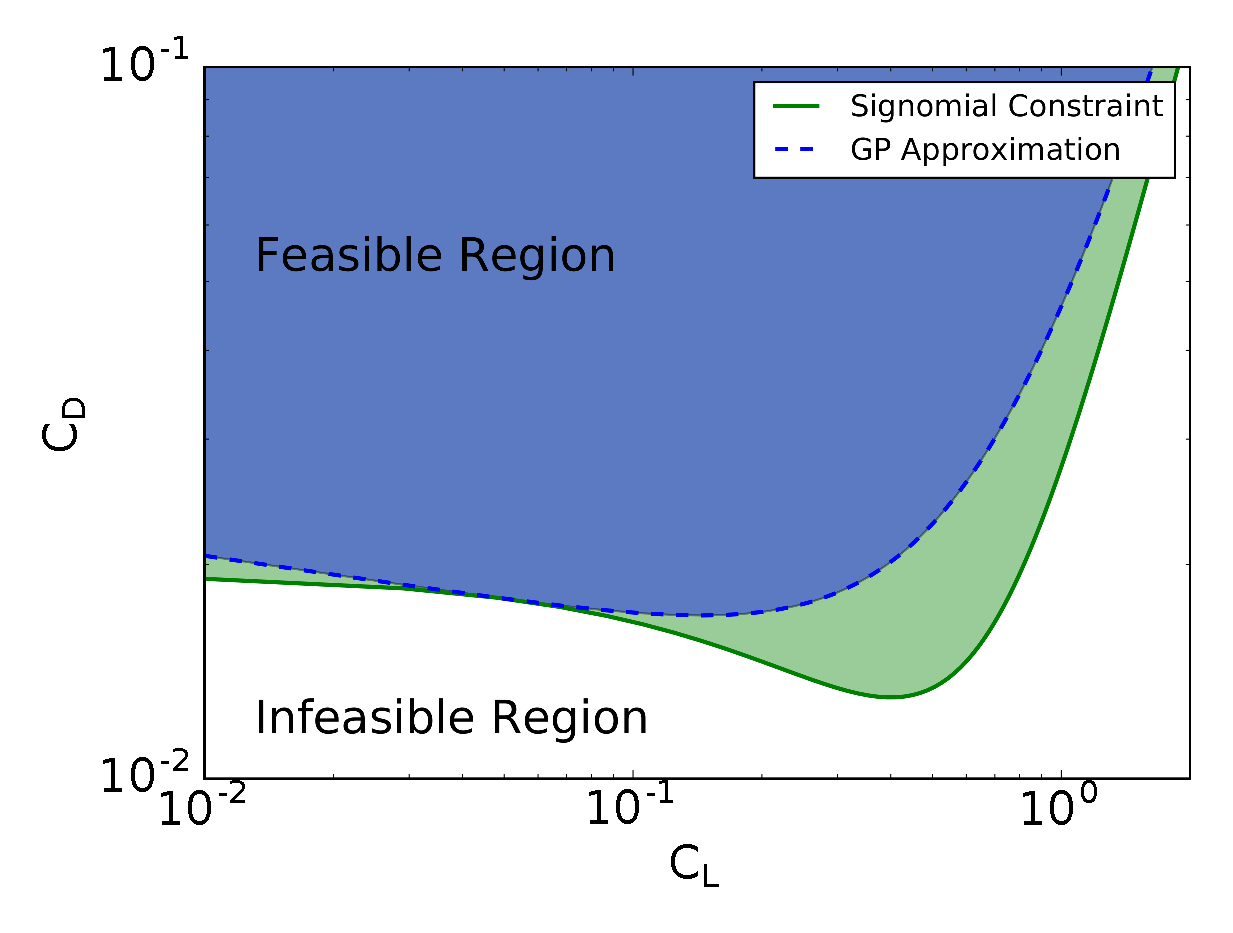
\includegraphics[width=0.9\linewidth]{posyapprox1.eps}
        \caption{Convex approximation about $C_{L} = 0.05$.}
    \end{subfigure}
    \begin{subfigure}[b]{0.5\linewidth}
        \centering
        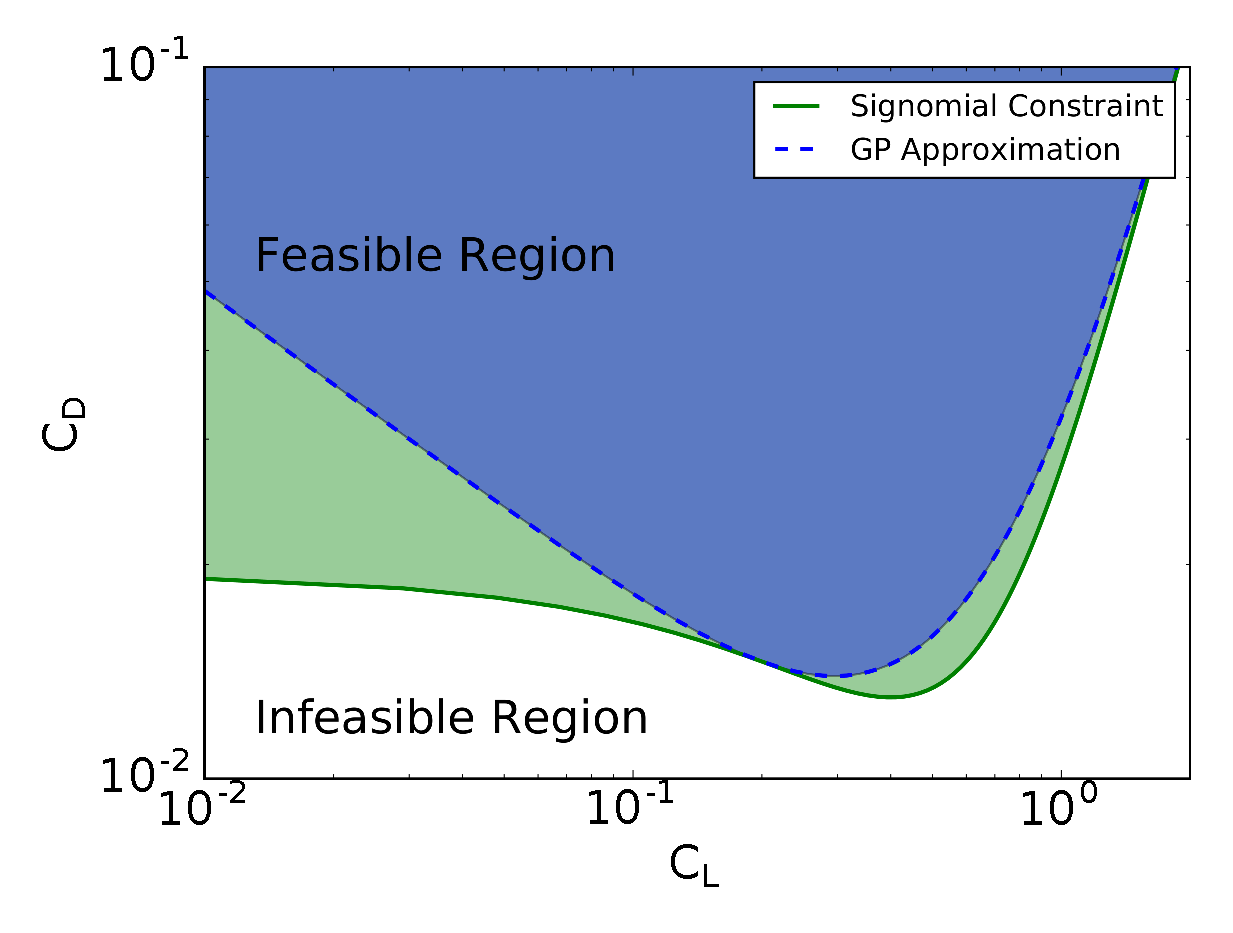
\includegraphics[width=0.9\linewidth]{posyapprox3.eps}
        \caption{Convex approximation about $C_{L} = 0.20.$}
    \end{subfigure}
    \caption{A signomial inequality constraint and GP approximations about two
different points.}
    \label{f:GPapproxs}
\end{figure*}

Signomial equality constraints can be approximated by monomials as shown in
Figure~\ref{f:sigeq} and may require a trust region. Trust regions were not
used in the presented model. Signomial equalities are the least desirable type
of constraint due the approximations involved. Most constraints in this work
were relaxed to inequalities and checked for tightness by GPkit~\cite{gpkit}. For
additional details on how signomial equalities are approximated, see Opgenoord
et al.~\cite{sigeqpaper}.

\begin{figure}[!ht]
\centering
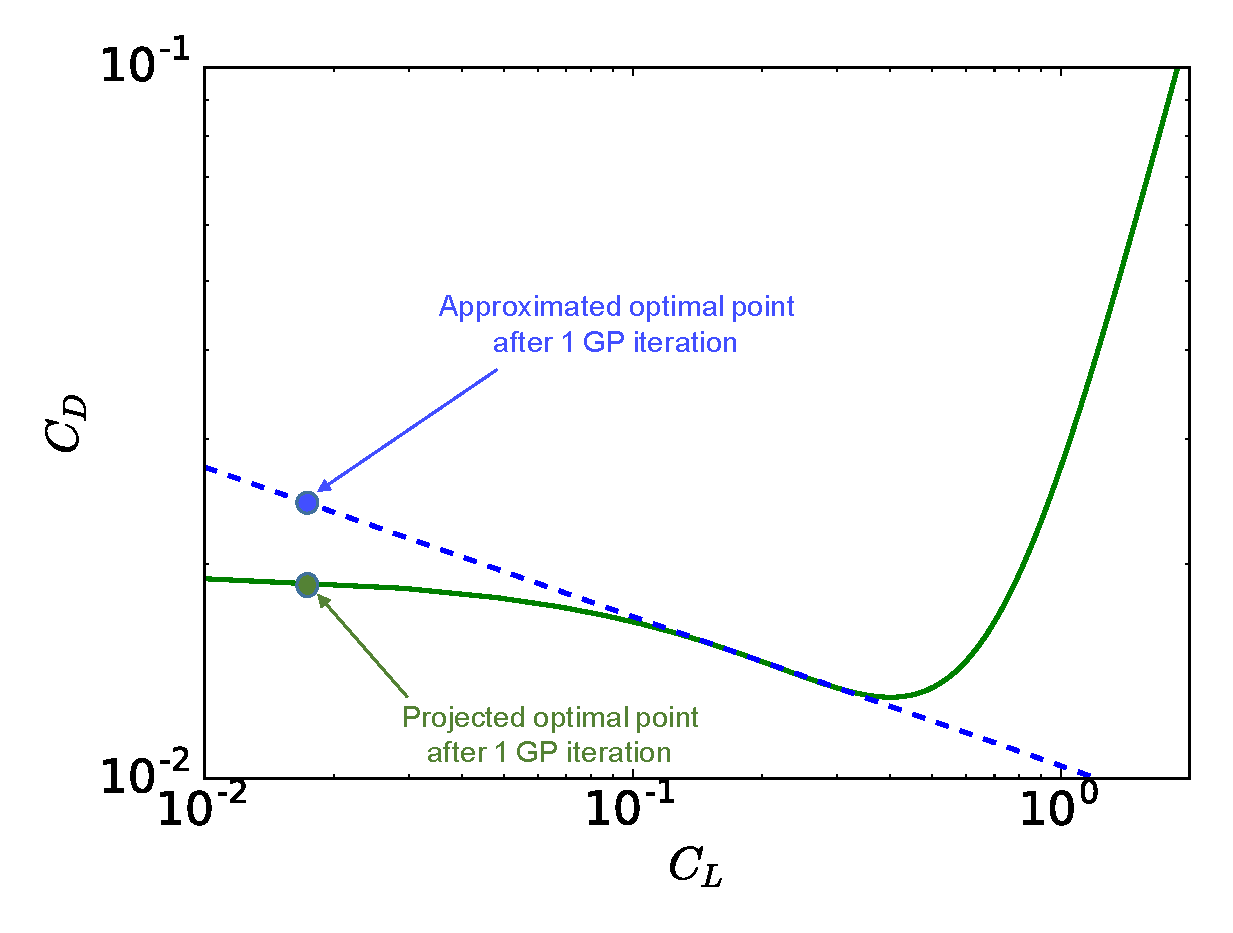
\includegraphics[width=0.5\linewidth]{sigeqapprox.eps}
\caption{The signomial equality constraint $C_{D} = f(C_{L})$ and its
approximation.}\label{f:sigeq}
\end{figure}

\chapter{Model Resources}

\section{Flight segment model variables}
\label{a:flightprofilevars}

\begin{footnotesize}
    \begin{table}[H]
        \centering
        \begin{tabular}{l c l}
            \toprule
            Variable & Units & Description \\
            \midrule
            $\frac{dh}{dt}$  & $~\mathrm{\tfrac{m}{hr}}$ & climb rate \\
            $h$ & $~\mathrm{m}$ & segment flight altitude\\
            $h_{avg}$ & $~\mathrm{m}$ & segment average flight altitude\\
            $R_s$ & $~\mathrm{km}$ & segment range\\
            $W_{start}$  & $~\mathrm{N}$ & segment beginning weight\\
            $W_{end}$ & $~\mathrm{N}$ & segment end weight\\
            $W_{avg}$ & $~\mathrm{N}$ & segment average weight\\
            $W_{f_s}$ & $~\mathrm{N}$ & segment fuel burn\\
            $W_{f_m}$  & $~\mathrm{N}$ & total mission fuel\\
            $t_s$ & $~\mathrm{hr}$ & segment time\\
            $t_m$  & $~\mathrm{hr}$ & total mission time\\
            \bottomrule
        \end{tabular}
        \caption{Variables introduced in the flight segment model.}
        \label{t:vars_flightprofile}
    \end{table}
\end{footnotesize}

%% This defines the bibliography file (main.bib) and the bibliography style.
%% If you want to create a bibliography file by hand, change the contents of
%% this file to a `thebibliography' environment.  For more information 
%% see section 4.3 of the LaTeX manual.
\begin{singlespace}
\bibliography{main}
\bibliographystyle{plain}
\end{singlespace}

\end{document}

